%!TEX root = ../final-report.tex
\chapter{Results}
\label{ch:results}

This chapter presents results for the four solvers. For each of the five initial conditions, the solvers will be compared for a few representative bathymetries. Reference results were obtained using the unbalanced solver from Section~\ref{sec:roe} on a very fine grid of 10,000 cells. At the end, the execution time of the different solvers is compared as well.

\section{Still Water}

\begin{figure}
  \centering
  \begin{subfigure}{\textwidth}
    %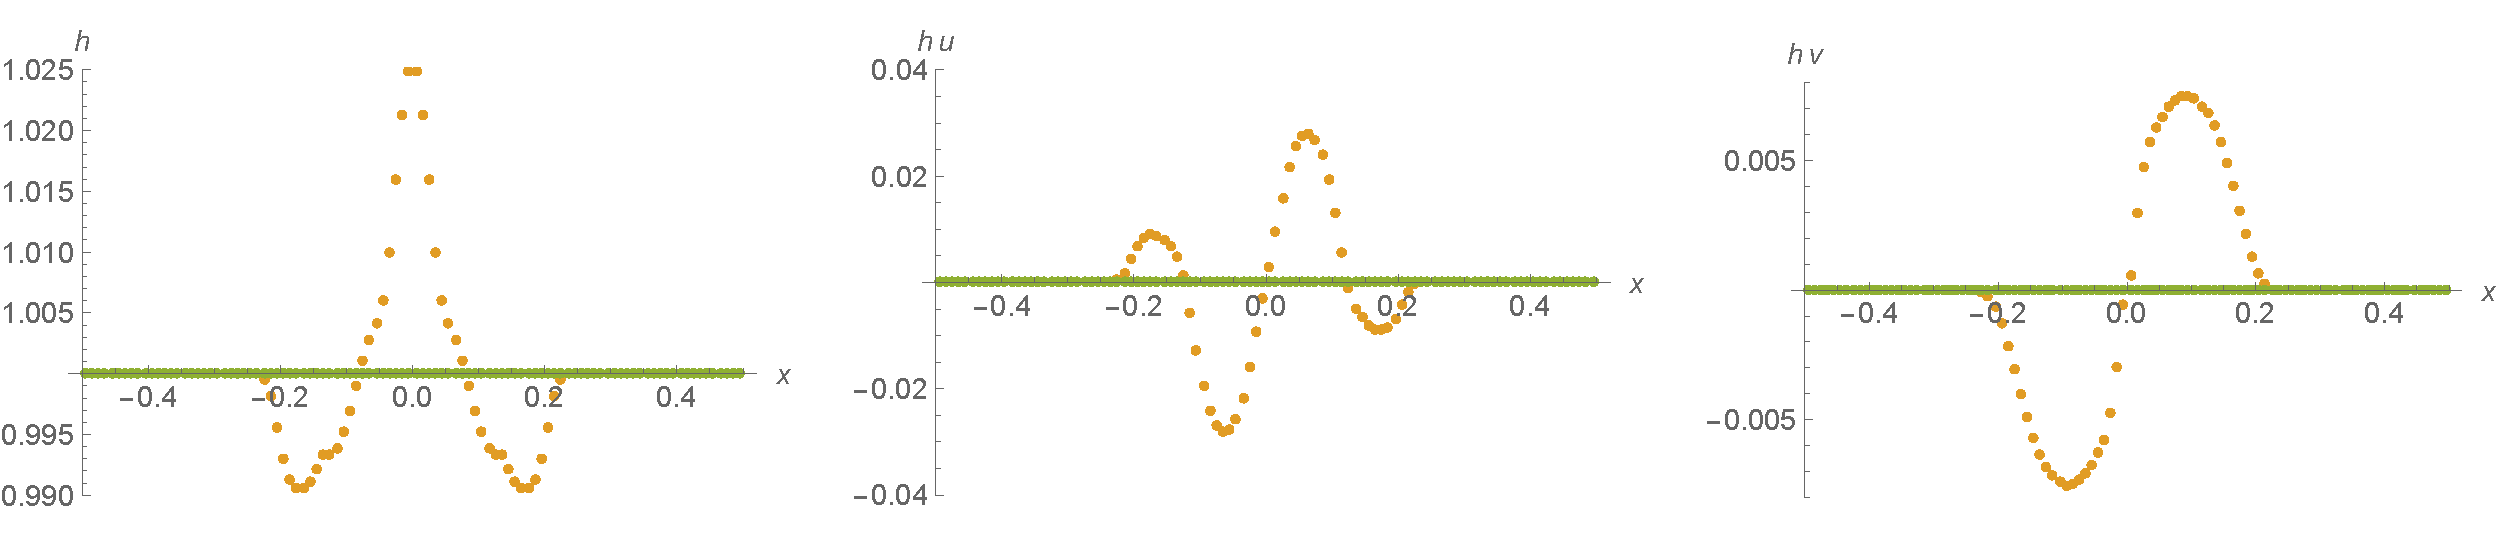
\includegraphics[width=\textwidth]{diagrams/results-still-1}
    \caption{$t = 0.1$}
    \label{fig:results-still-1}
  \end{subfigure} \\
  \begin{subfigure}{\textwidth}
    %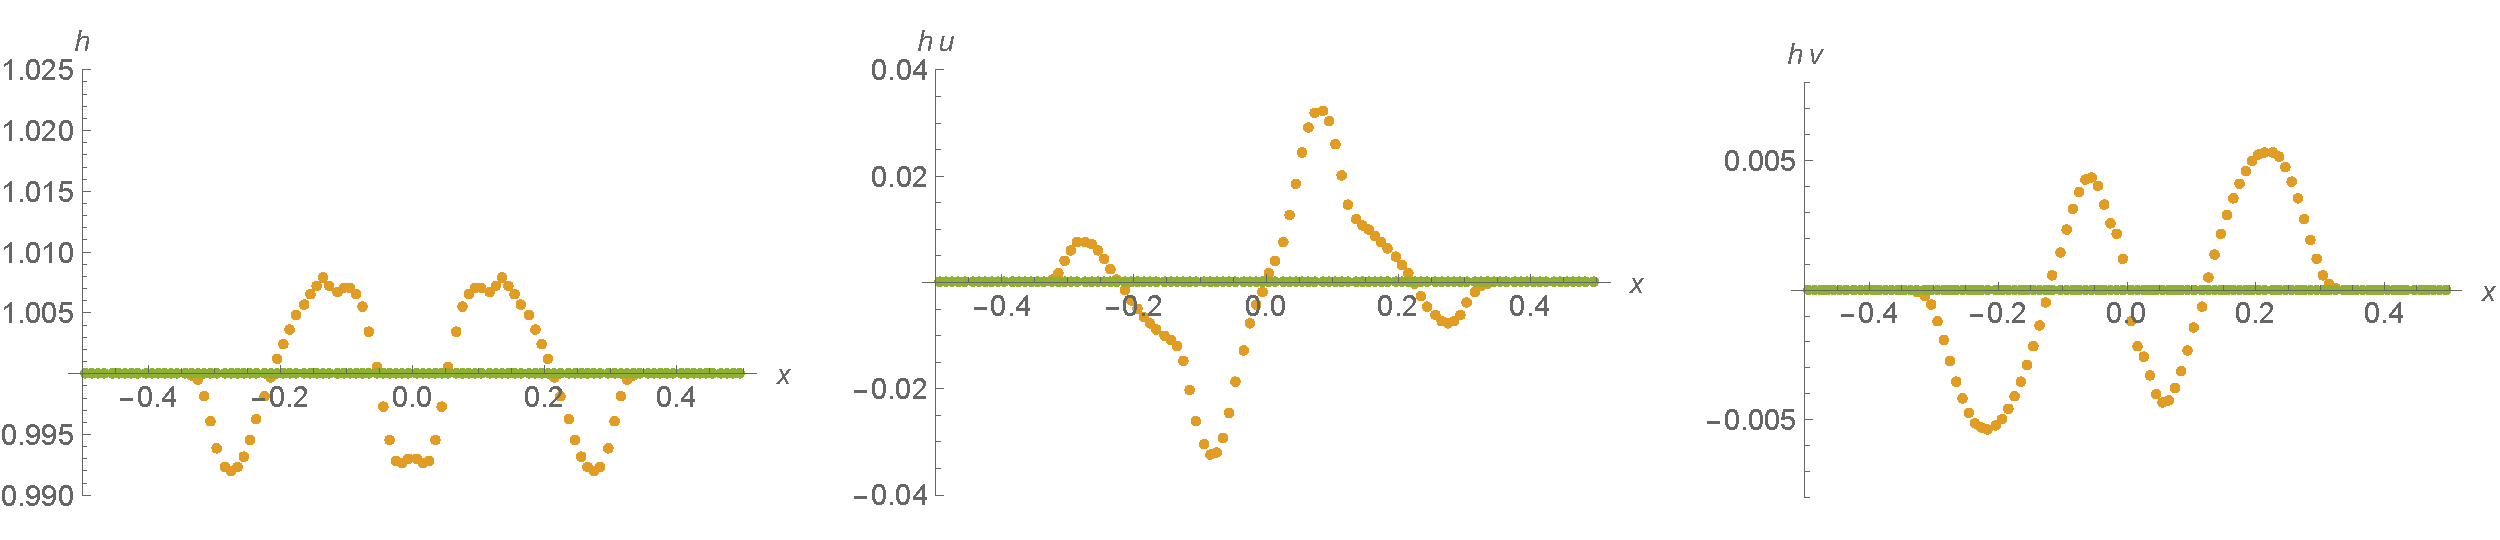
\includegraphics[width=\textwidth]{diagrams/results-still-2}
    \caption{$t = 0.2$}
    \label{fig:results-still-2}
  \end{subfigure} \\
  \begin{subfigure}{\textwidth}
    %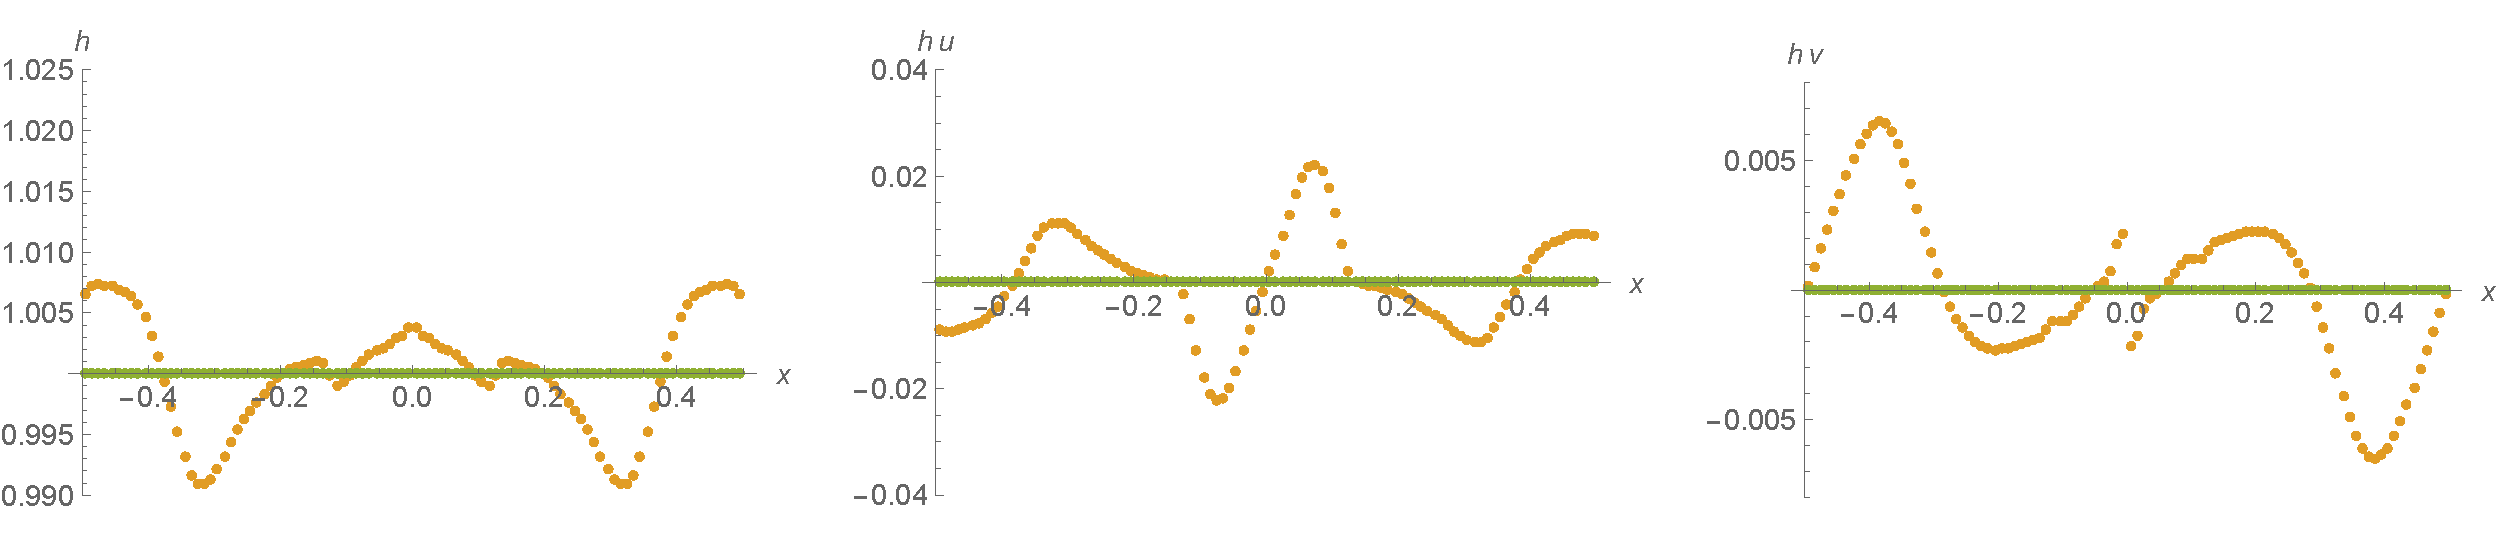
\includegraphics[width=\textwidth]{diagrams/results-still-5}
    \caption{$t = 0.5$}
    \label{fig:results-still-5}
  \end{subfigure} \\
  \begin{subfigure}{\textwidth}
    %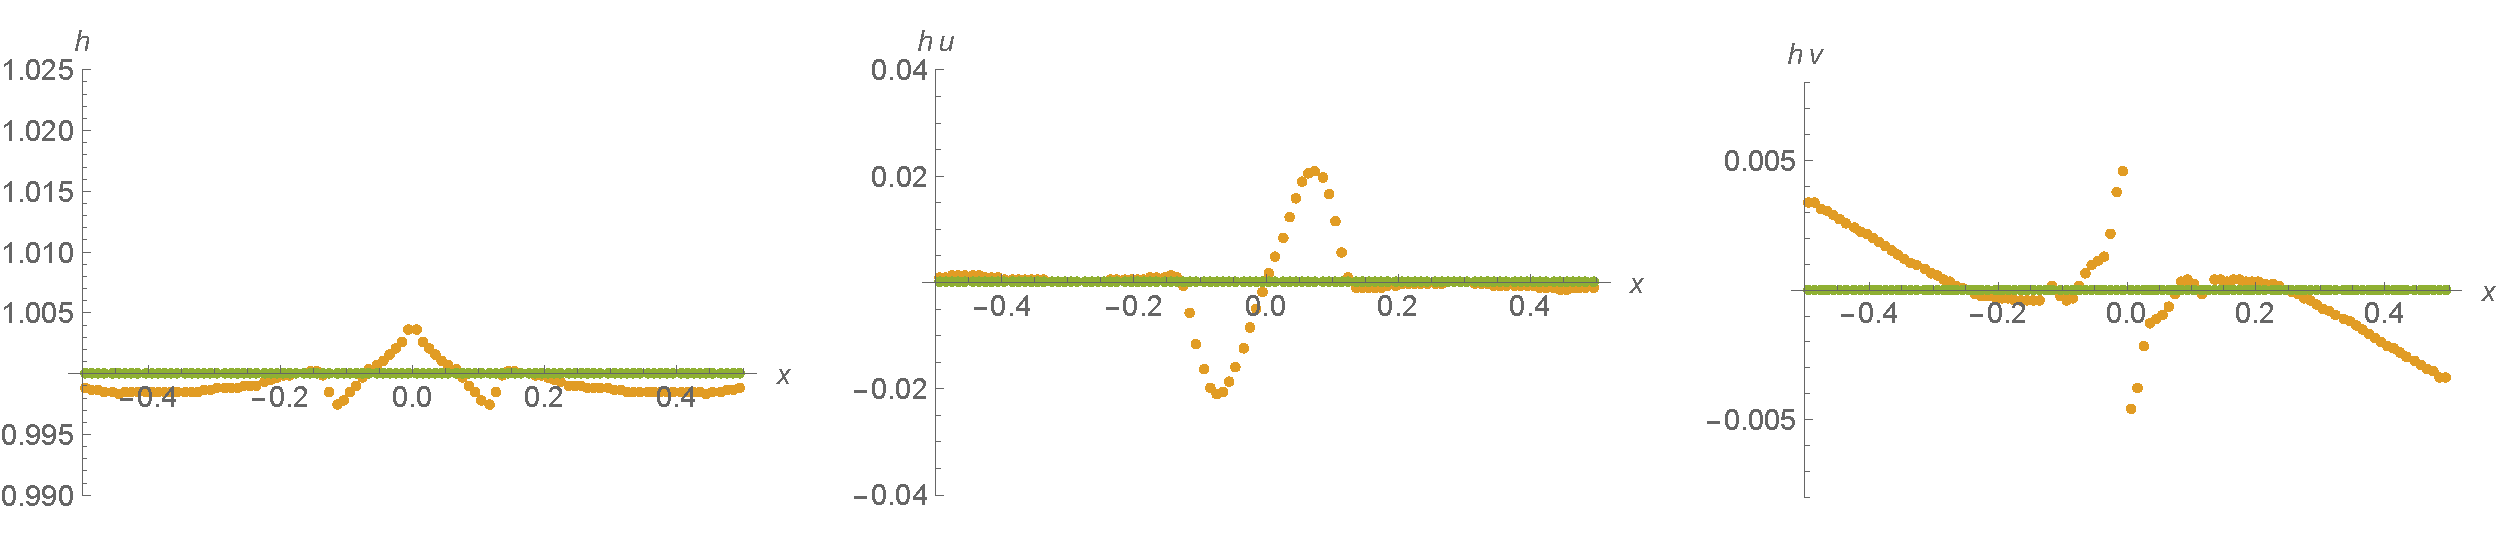
\includegraphics[width=\textwidth]{diagrams/results-still-10}
    \caption{$t = 1.0$}
    \label{fig:results-still-10}
  \end{subfigure}
  \caption{Results for still water over a cosine ridge. The exact solution is $h = 1$, $hu = hv = 0$ for all times. The orange data was obtained with the unbalanced solver over 100 grid cells. The green data corresponds to any of the three balanced solvers. The columns correspond to the conserved variables $h$, $hu$ and $hv$ and the rows to different time levels. $K = 10$.}
  \label{fig:results-still}
\end{figure}

The first system is simply still water over a cosine ridge, as shown in Fig.~\ref{fig:bath-cosine}. Figs~\ref{fig:results-still} show the results at times $t \in \{0.1, 0.2, 0.5, 1.0\}$. Only one set of data has been included for the three balanced solvers, as they are indistinguishable in the plot. All sets of data have been obtained for 100 grid cells and with $K = 10$.

Of course, these plots show exactly the motivation for developing balanced solvers in the first place: the unbalanced solver develops quite substantial waves, about 1\% of the water depth, and settles into a state which is not still with errors of about 0.5\%. From inspection across different grid sizes it appears that the size of the waves is proportional to $1/N$, whereas the error in the settled state is proportional to $1/N^2$.

It should be noted that the data for the two rogers solvers is exactly zero (since all terms that appear anywhere in the method are always zero), whereas the LeVeque solver is only zero to machine precision (since it relies on two separate computations to make the Riemann problems at the cell edges disappear).

\section{Wave through Still Water}

\begin{figure}
  \centering
  \begin{subfigure}{\textwidth}
    %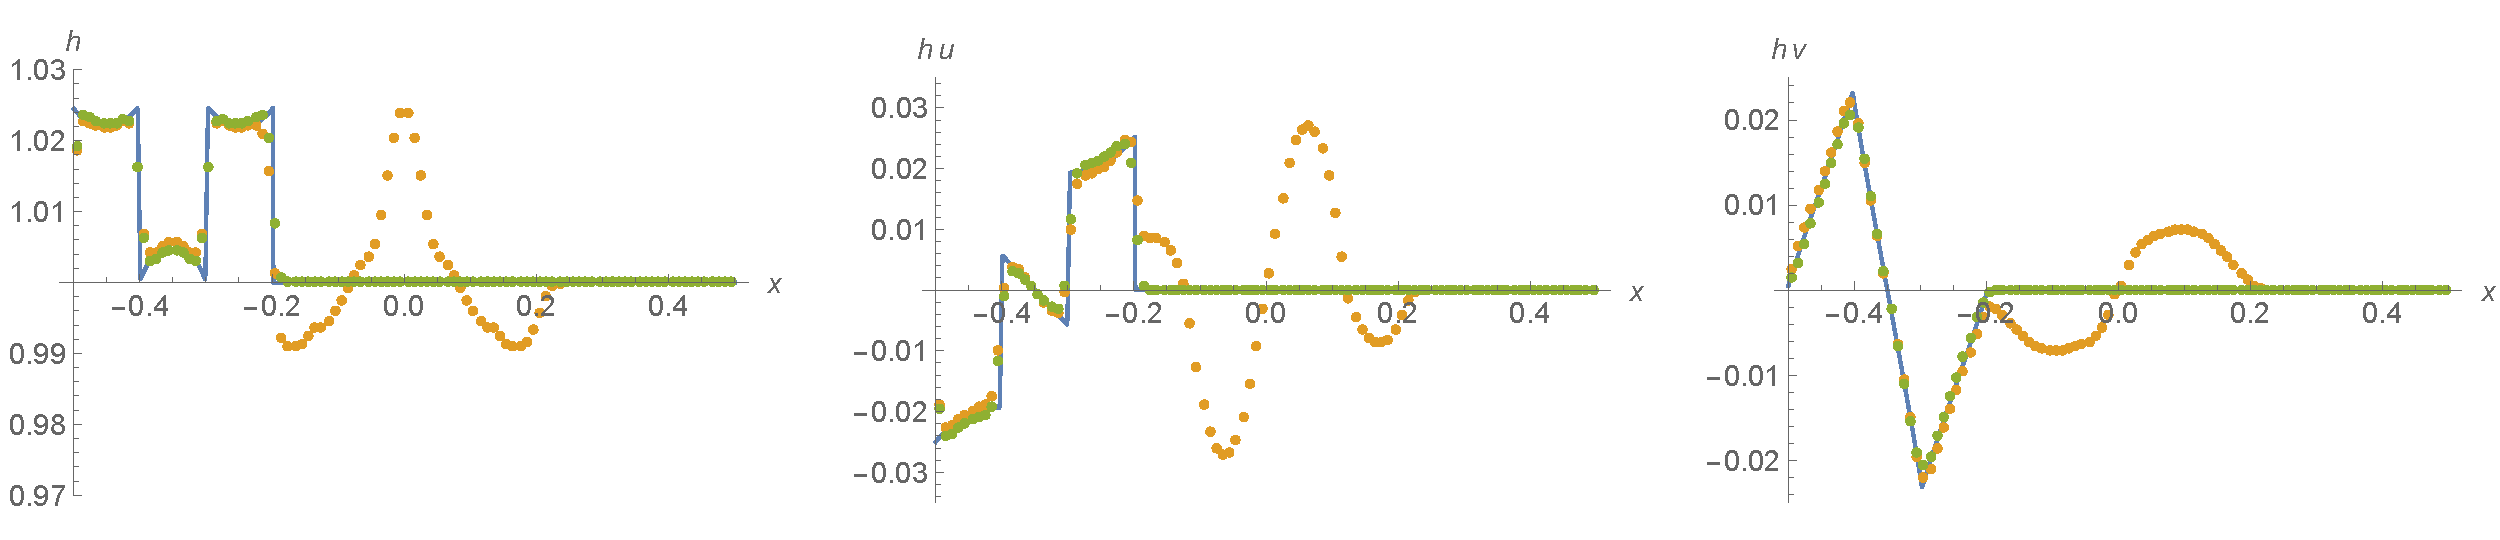
\includegraphics[width=\textwidth]{diagrams/results-wave-lev-1}
    \caption{$t = 0.1$}
    \label{fig:results-wave-lev-1}
  \end{subfigure} \\
  \begin{subfigure}{\textwidth}
    %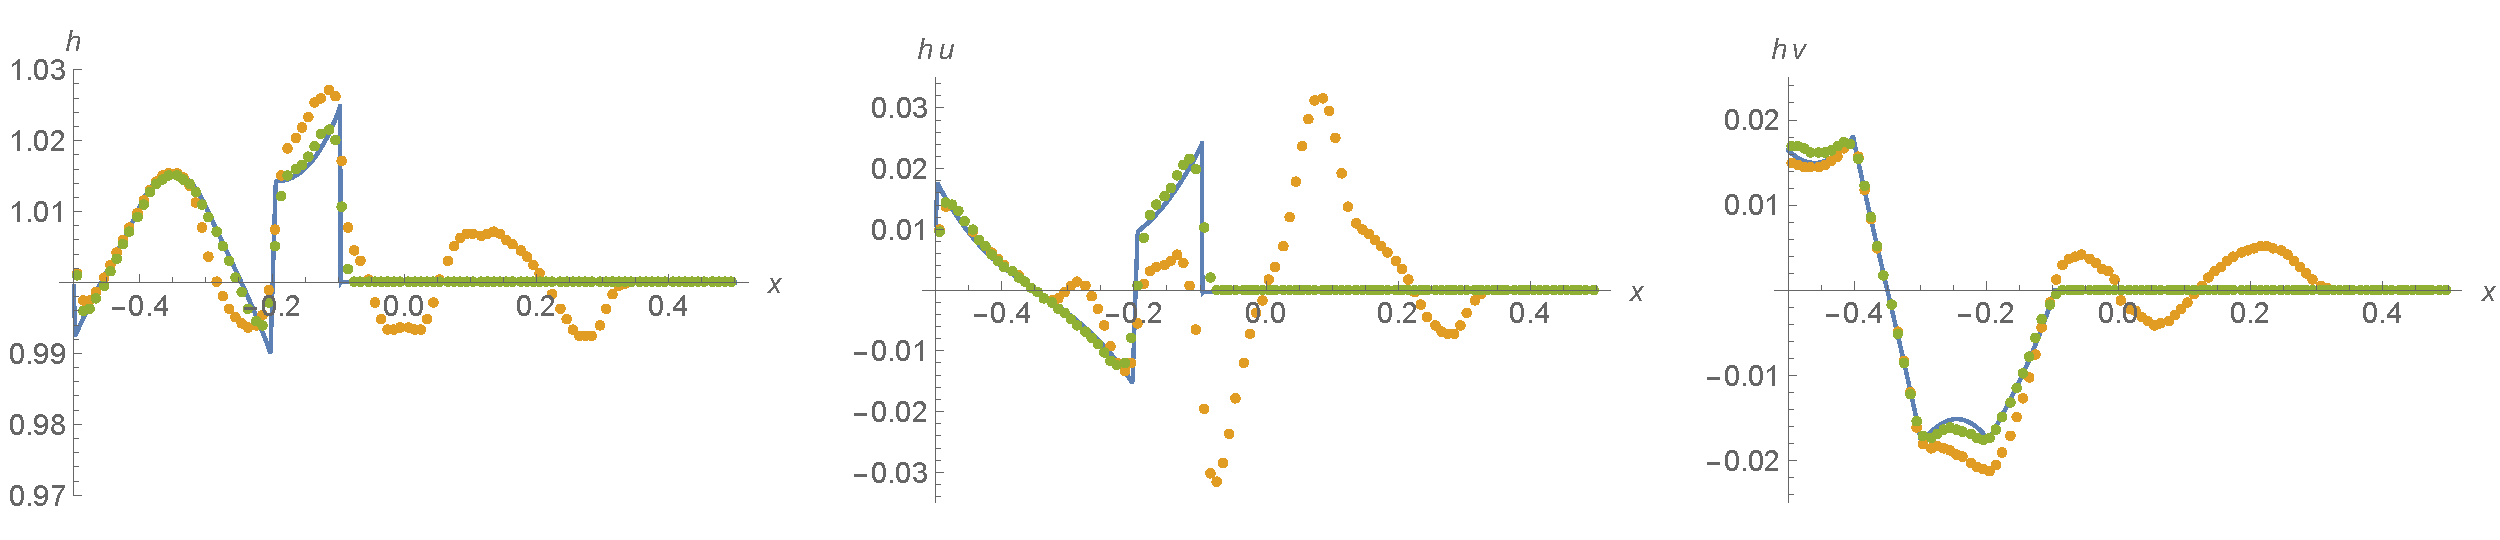
\includegraphics[width=\textwidth]{diagrams/results-wave-lev-2}
    \caption{$t = 0.2$}
    \label{fig:results-wave-lev-2}
  \end{subfigure} \\
  \begin{subfigure}{\textwidth}
    %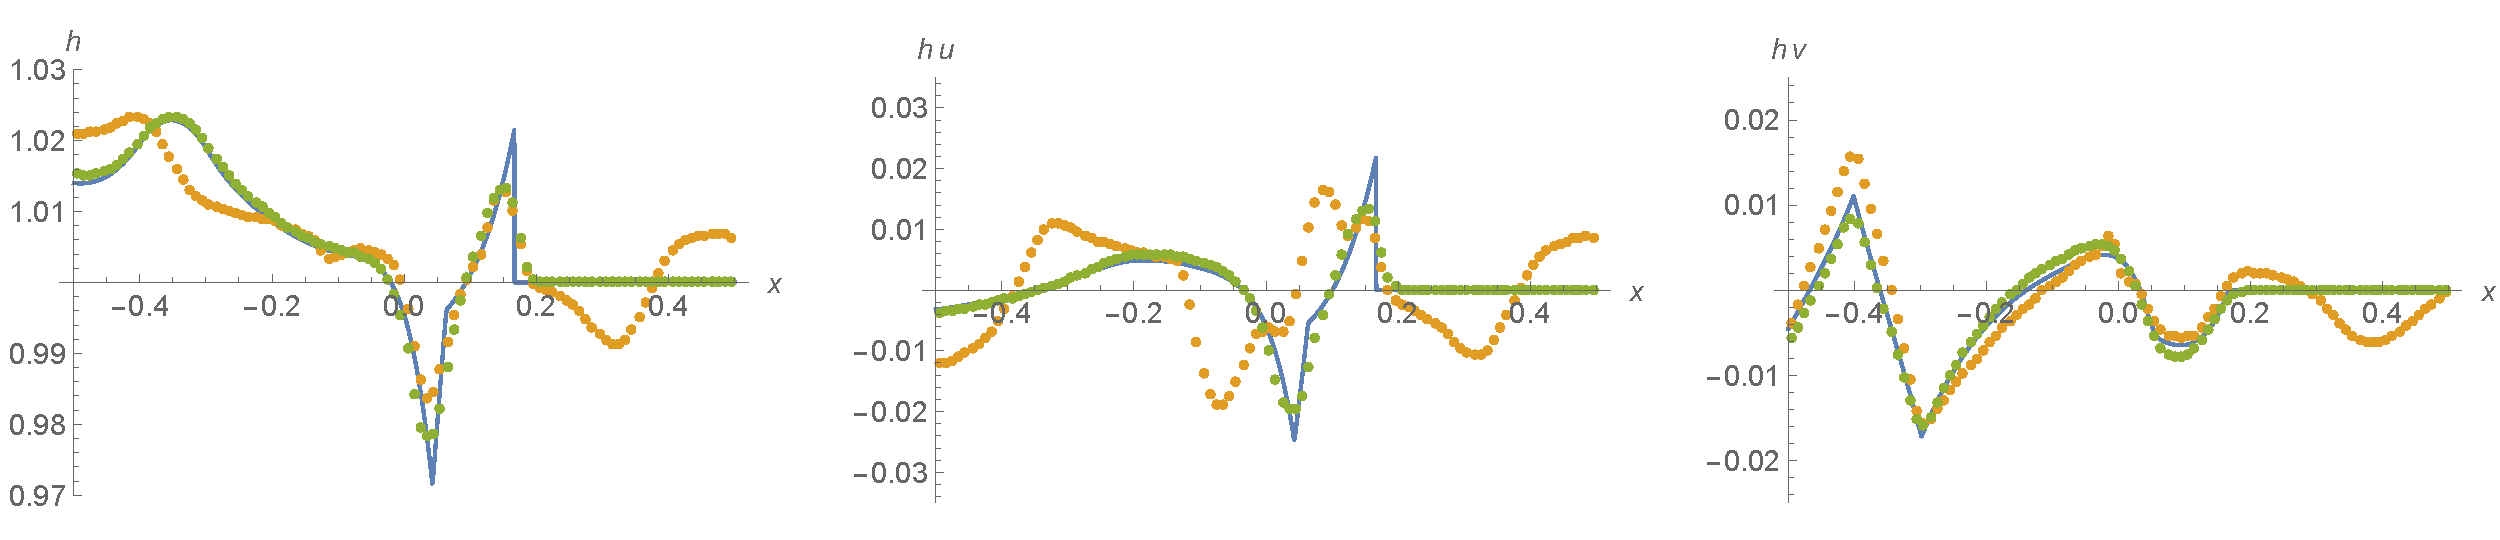
\includegraphics[width=\textwidth]{diagrams/results-wave-lev-5}
    \caption{$t = 0.5$}
    \label{fig:results-wave-lev-5}
  \end{subfigure} \\
  \begin{subfigure}{\textwidth}
    %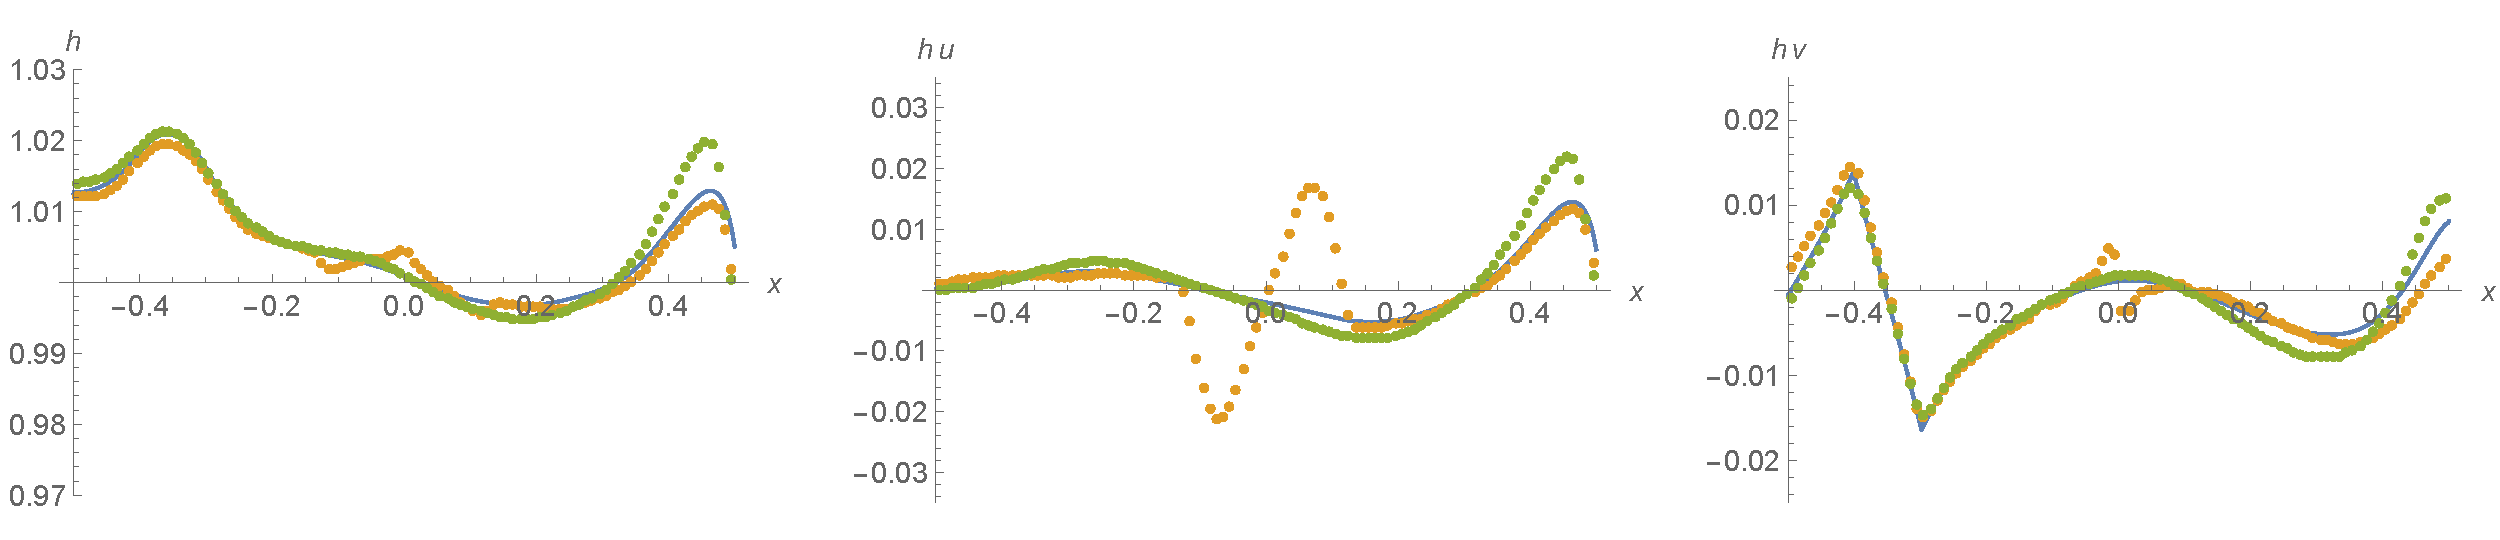
\includegraphics[width=\textwidth]{diagrams/results-wave-lev-10}
    \caption{$t = 1.0$}
    \label{fig:results-wave-lev-10}
  \end{subfigure}
  \caption{Results for wave through still water over a cosine ridge. The reference solution has been computed with the unbalanced solver on 10000 grid cells and is shown as a solid blue line. The orange data was obtained with the unbalanced solver over 100 grid cells. The green data corresponds to the LeVeque solver. The columns correspond to the conserved variables $h$, $hu$ and $hv$ and the rows to different time levels. $K = 10$.}
  \label{fig:results-wave-lev}
\end{figure}

\begin{figure}
  \centering
  \begin{subfigure}{\textwidth}
    %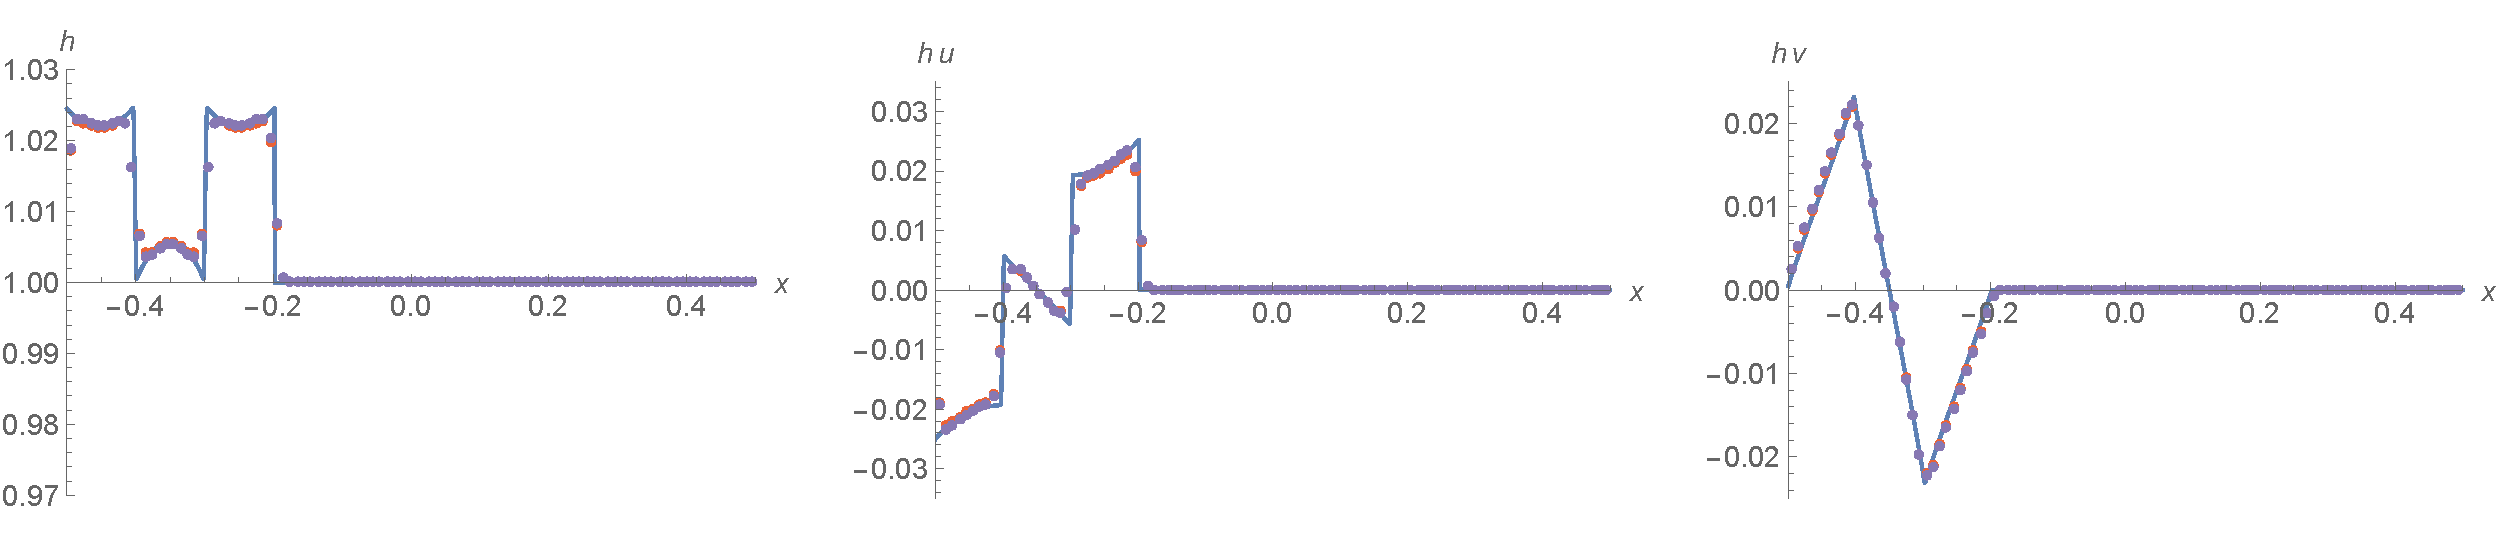
\includegraphics[width=\textwidth]{diagrams/results-wave-rog-1}
    \caption{$t = 0.1$}
    \label{fig:results-wave-rog-1}
  \end{subfigure} \\
  \begin{subfigure}{\textwidth}
    %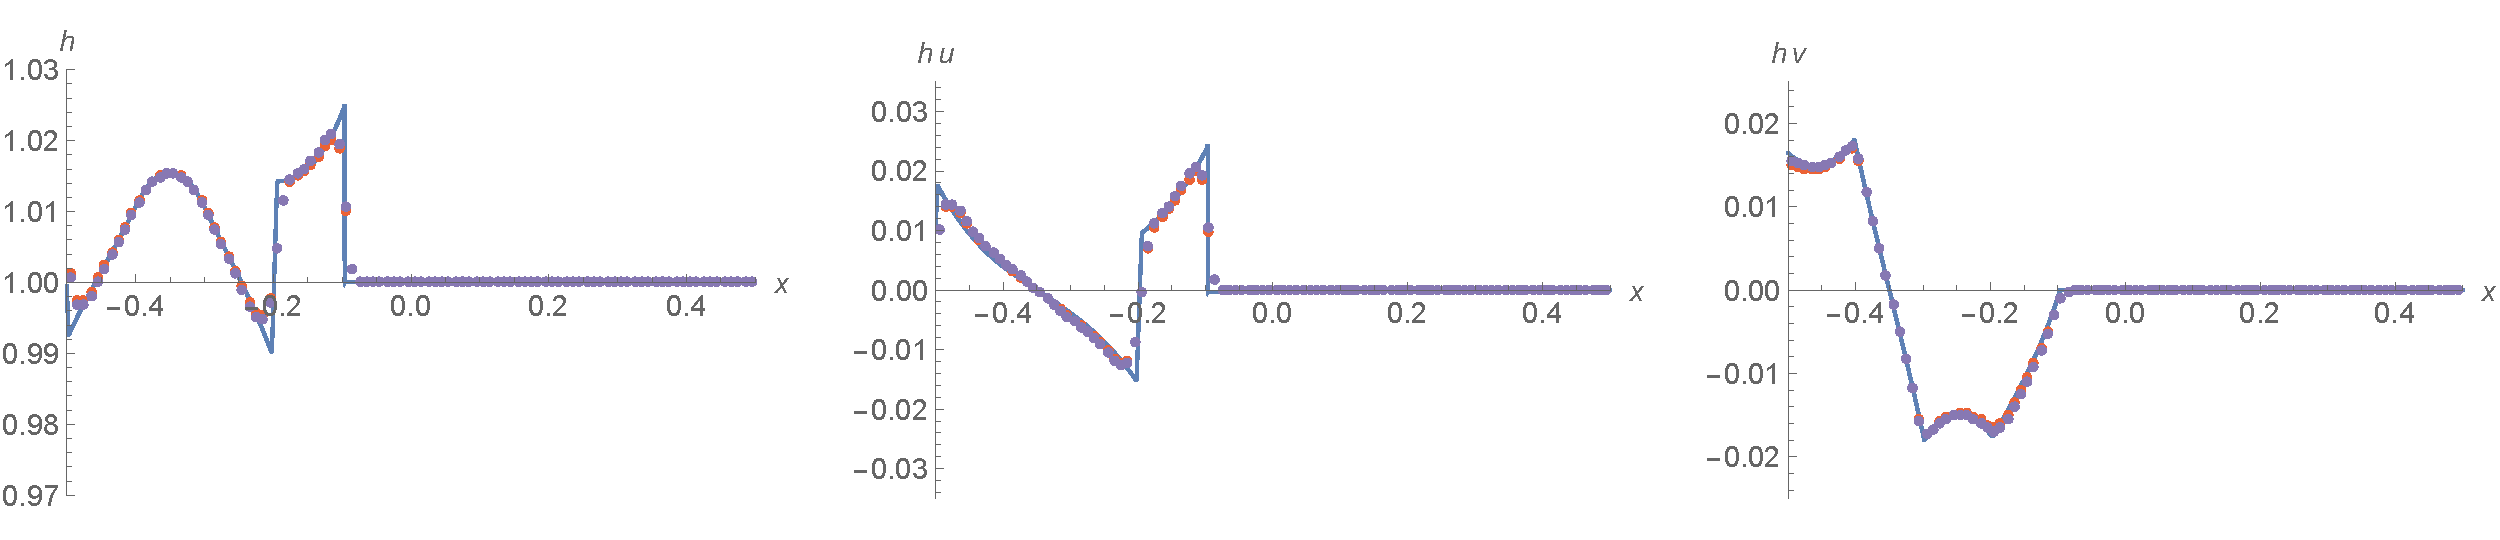
\includegraphics[width=\textwidth]{diagrams/results-wave-rog-2}
    \caption{$t = 0.2$}
    \label{fig:results-wave-rog-2}
  \end{subfigure} \\
  \begin{subfigure}{\textwidth}
    %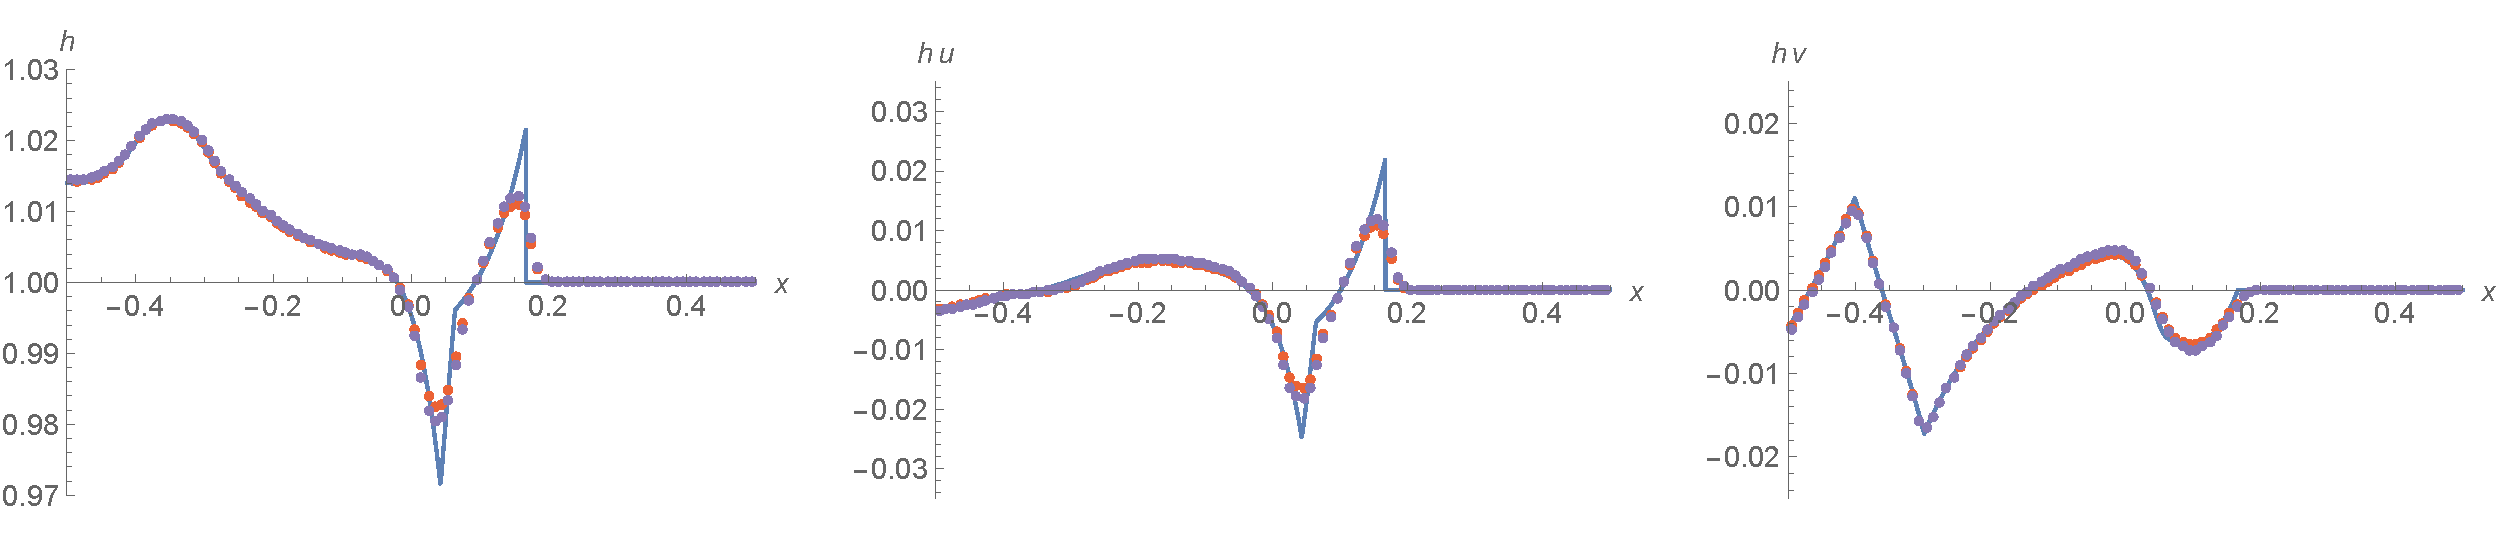
\includegraphics[width=\textwidth]{diagrams/results-wave-rog-5}
    \caption{$t = 0.5$}
    \label{fig:results-wave-rog-5}
  \end{subfigure} \\
  \begin{subfigure}{\textwidth}
    %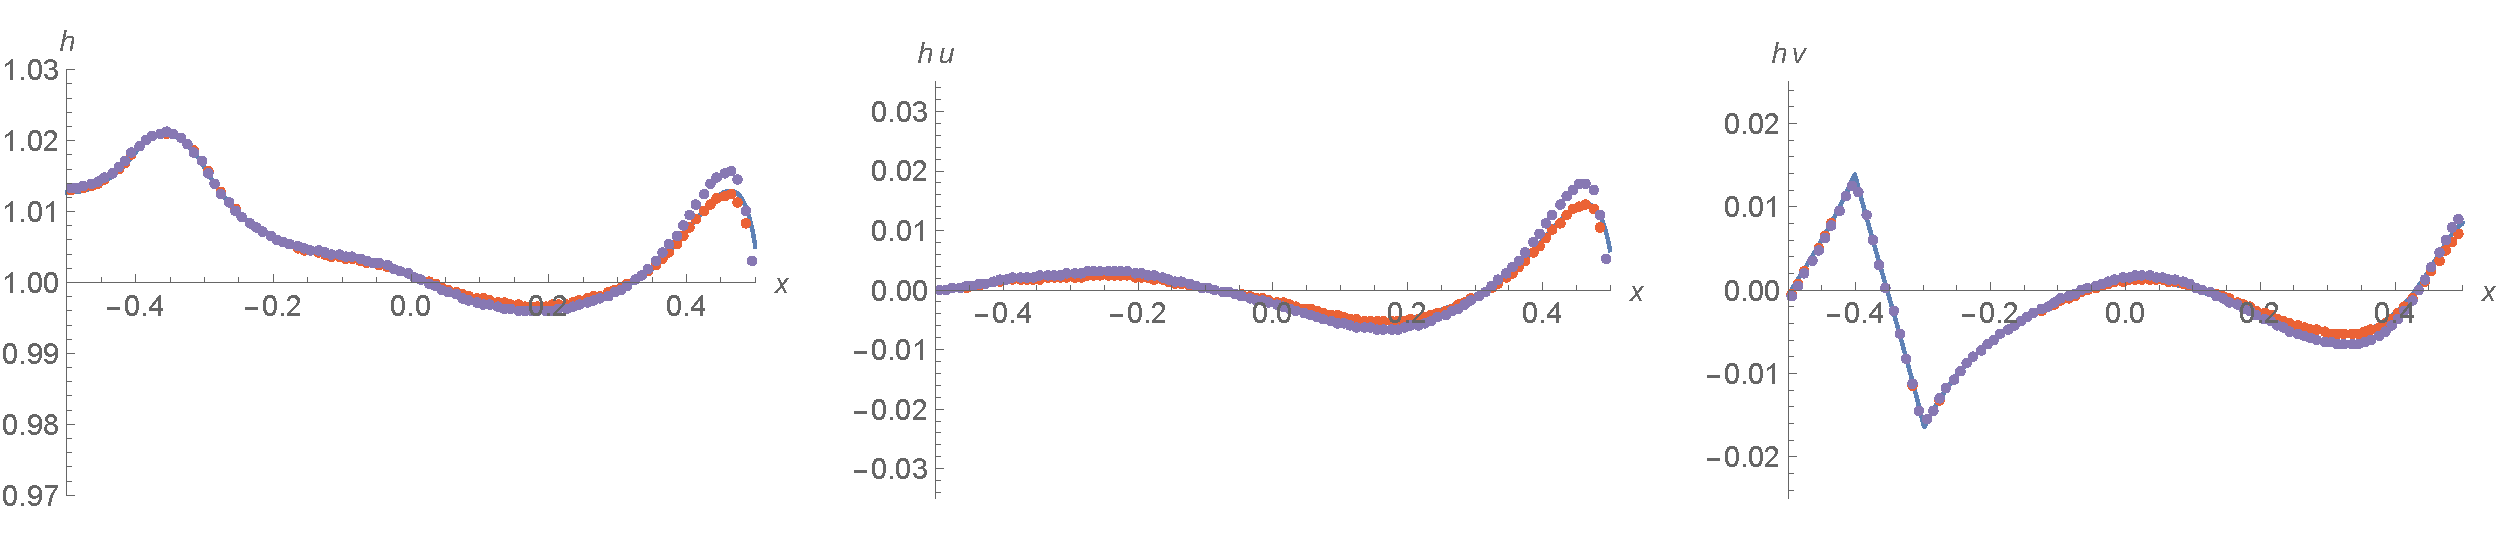
\includegraphics[width=\textwidth]{diagrams/results-wave-rog-10}
    \caption{$t = 1.0$}
    \label{fig:results-wave-rog-10}
  \end{subfigure}
  \caption{Results for wave through still water over a cosine ridge. The reference solution has been computed with the unbalanced solver on 10000 grid cells and is shown as a solid blue line. The red data was obtained with the Rogers solver for still water systems over 100 grid cells. The blue data corresponds to the Rogers solver for geostrophic equilibria. The columns correspond to the conserved variables $h$, $hu$ and $hv$ and the rows to different time levels. $K = 10$.}
  \label{fig:results-wave-rog}
\end{figure}

For this system a small perturbation is added to the surface profile of the water, near the left edge of the domain. The results for the unbalanced and LeVeque solver are shown in Figs.~\ref{fig:results-wave-lev}, those for the Rogers solvers in Figs.~\ref{fig:results-wave-rog}.

It is notable that the unphysical waves of the balanced solver are comparable to the size of the real waves at this resolution, which makes the results very unreliable.

The balanced solver are much better at approximating the real solution, and produce very good results, considering the low resolution. It is hard to compare the performance of the three balanced solvers in detail, but it seems that the LeVeque solver produces the least accurate result, whereas the Rogers solver for still water systems approximates the real solution most closely.

\section{Geostrophic Equilibrium}

\begin{figure}
  \centering
  \begin{subfigure}{\textwidth}
    %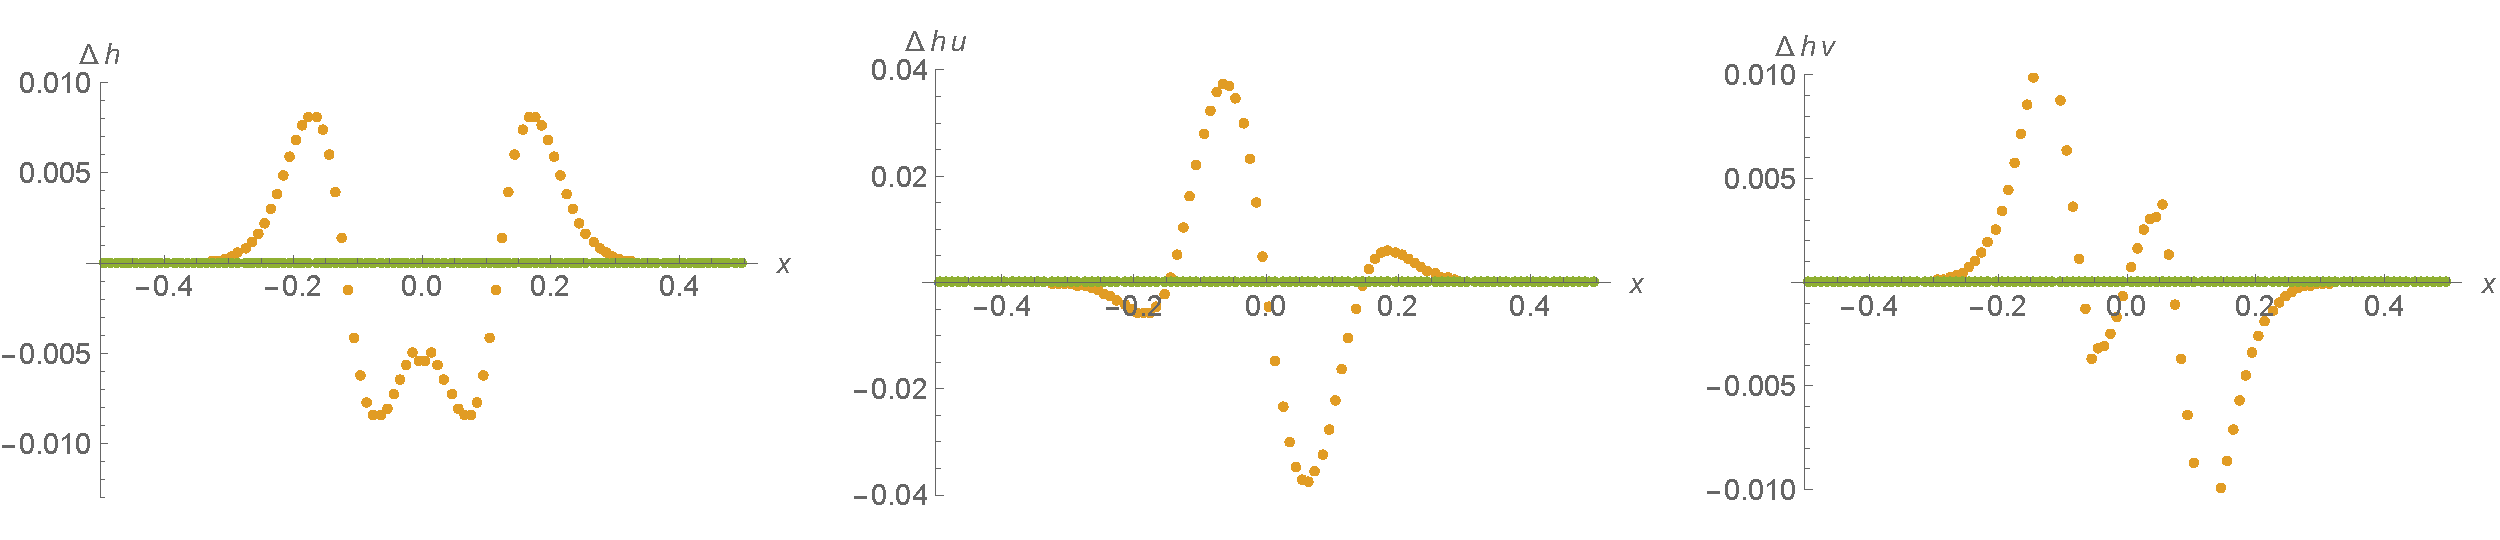
\includegraphics[width=\textwidth]{diagrams/results-geo-1}
    \caption{$t = 0.1$}
    \label{fig:results-geo-1}
  \end{subfigure} \\
  \begin{subfigure}{\textwidth}
    %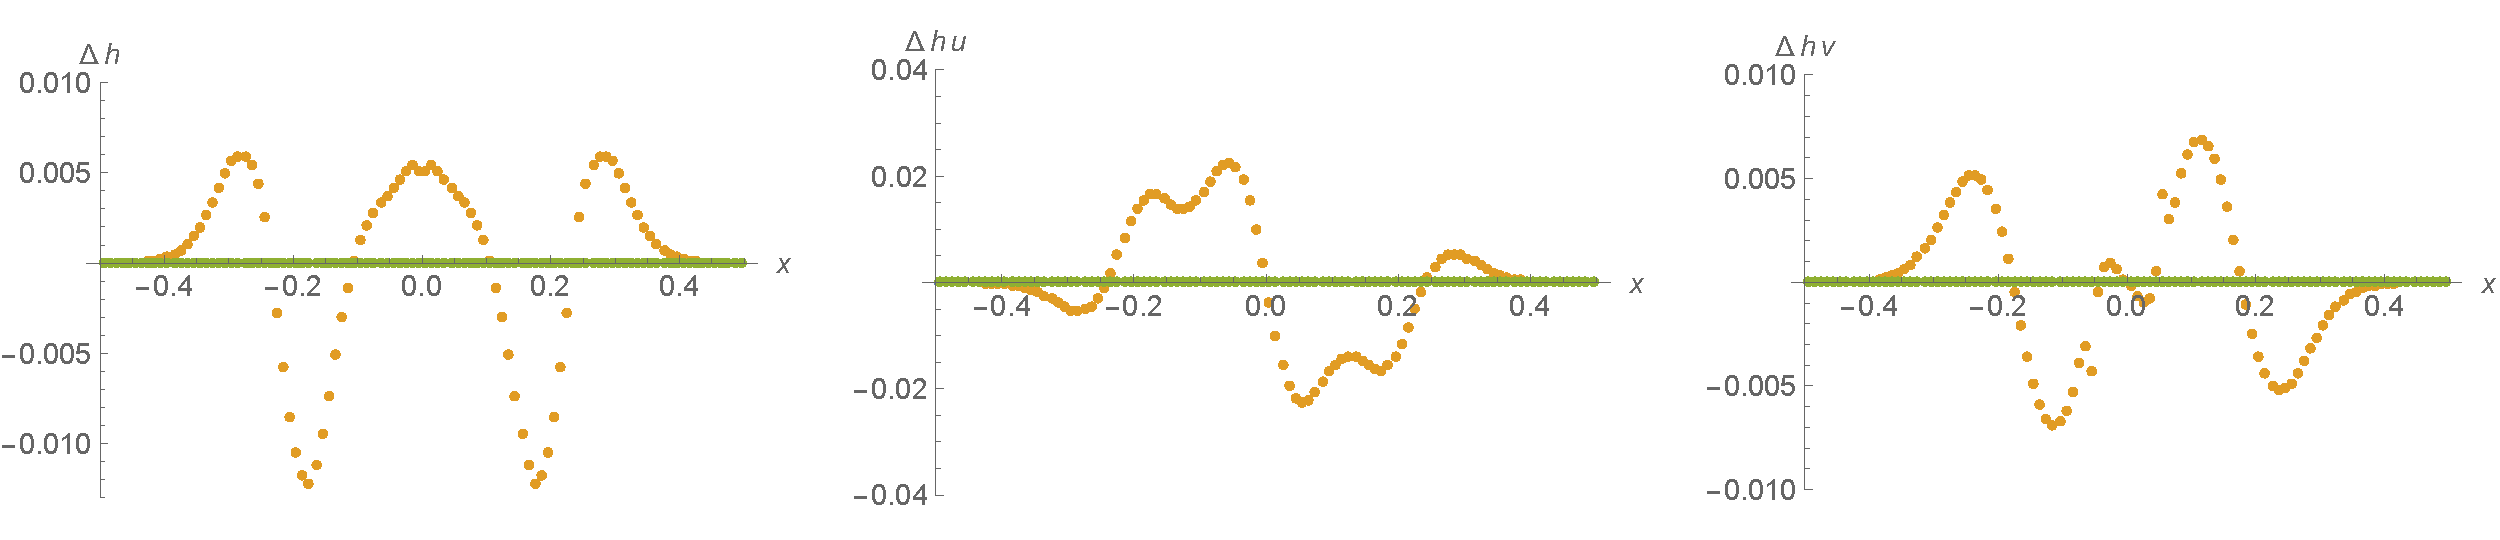
\includegraphics[width=\textwidth]{diagrams/results-geo-2}
    \caption{$t = 0.2$}
    \label{fig:results-geo-2}
  \end{subfigure} \\
  \begin{subfigure}{\textwidth}
    %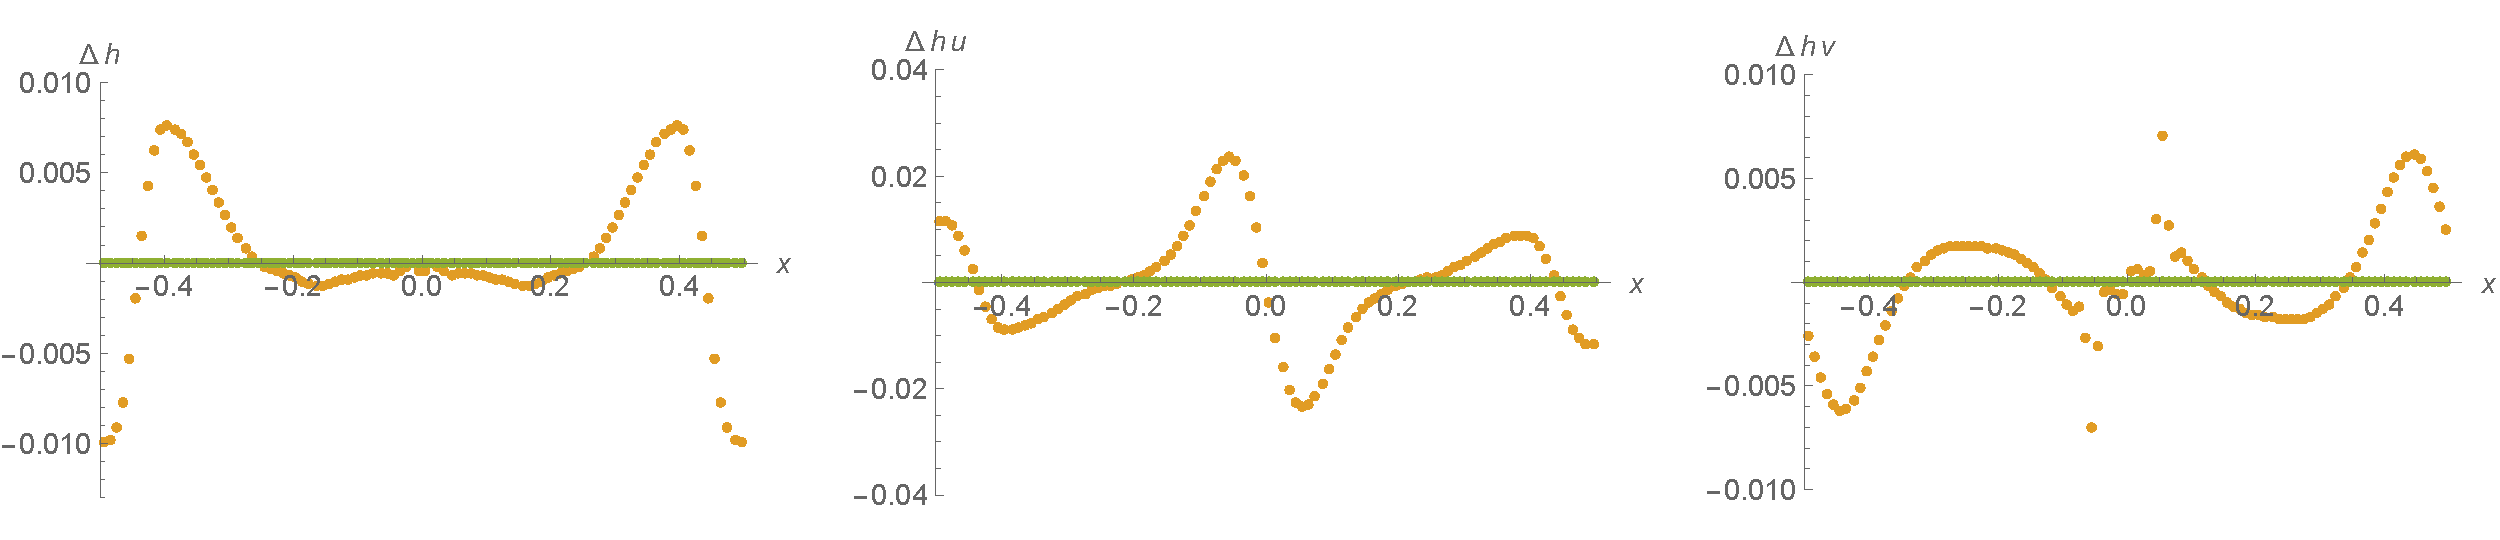
\includegraphics[width=\textwidth]{diagrams/results-geo-5}
    \caption{$t = 0.5$}
    \label{fig:results-geo-5}
  \end{subfigure} \\
  \begin{subfigure}{\textwidth}
    %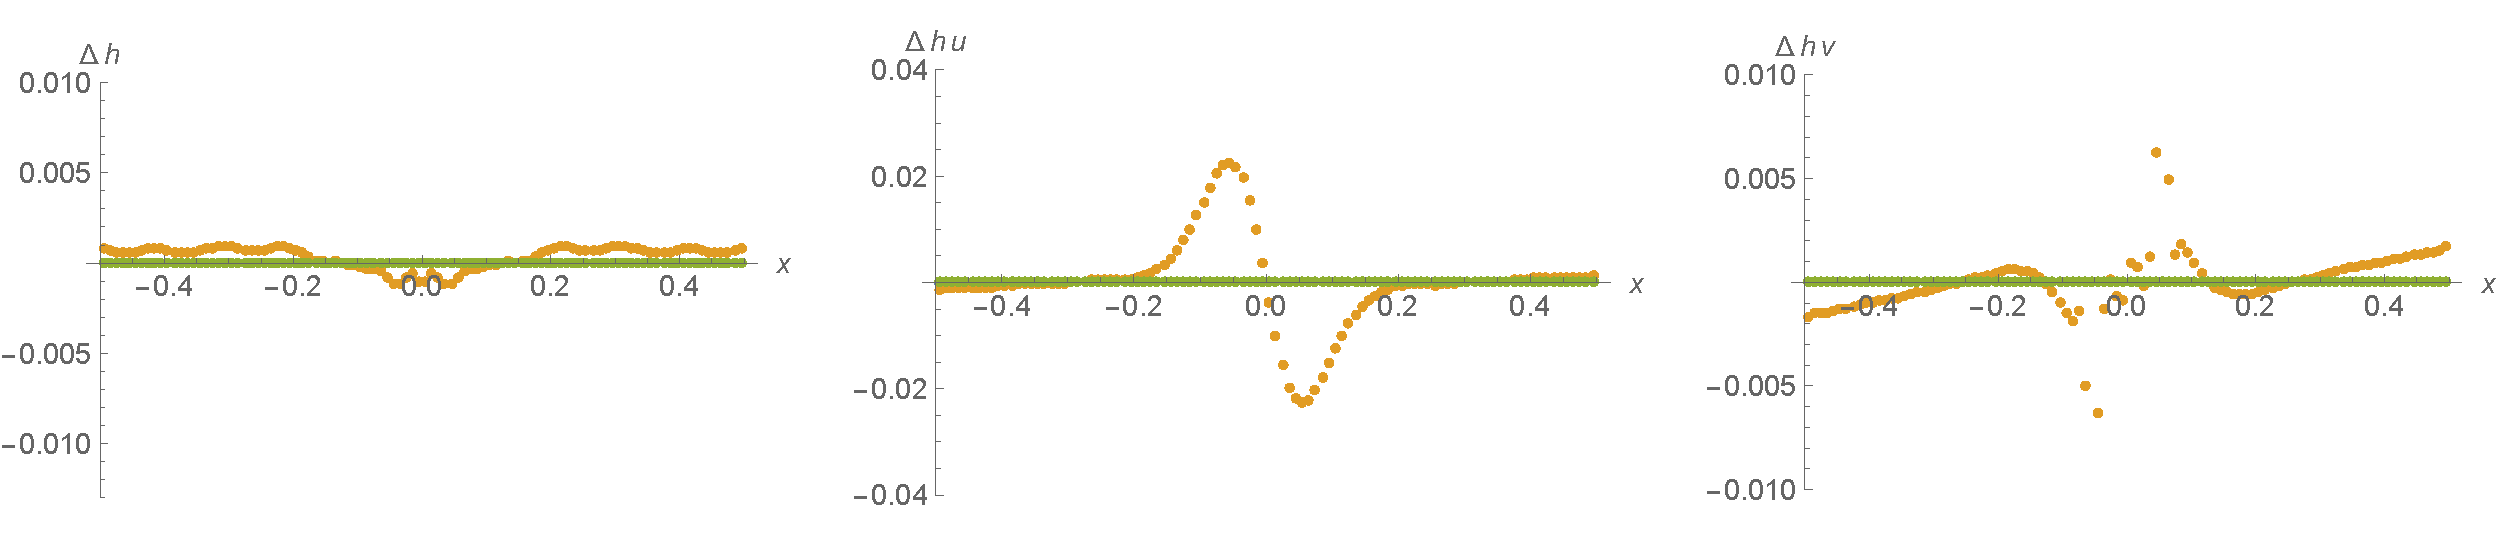
\includegraphics[width=\textwidth]{diagrams/results-geo-10}
    \caption{$t = 1.0$}
    \label{fig:results-geo-10}
  \end{subfigure}
  \caption{Results for geostrophic equilibrium. The equilibrium state has been subtracted off the plots, such that the exact solution is $\Delta h = \Delta hu = \Delta hv = 0$. The orange data corresponds to both the unbalanced solver and the Rogers solver for still water over 100 grid cells. The green data corresponds to both the LeVeque solver and the Rogers solver for geostrophic equilibria. The columns correspond to the deviations of the conserved variables $h$, $hu$ and $hv$ and the rows to different time levels. $K = 10$.}
  \label{fig:results-geo}
\end{figure}

\begin{figure}
  \centering
  \begin{subfigure}{\textwidth}
    %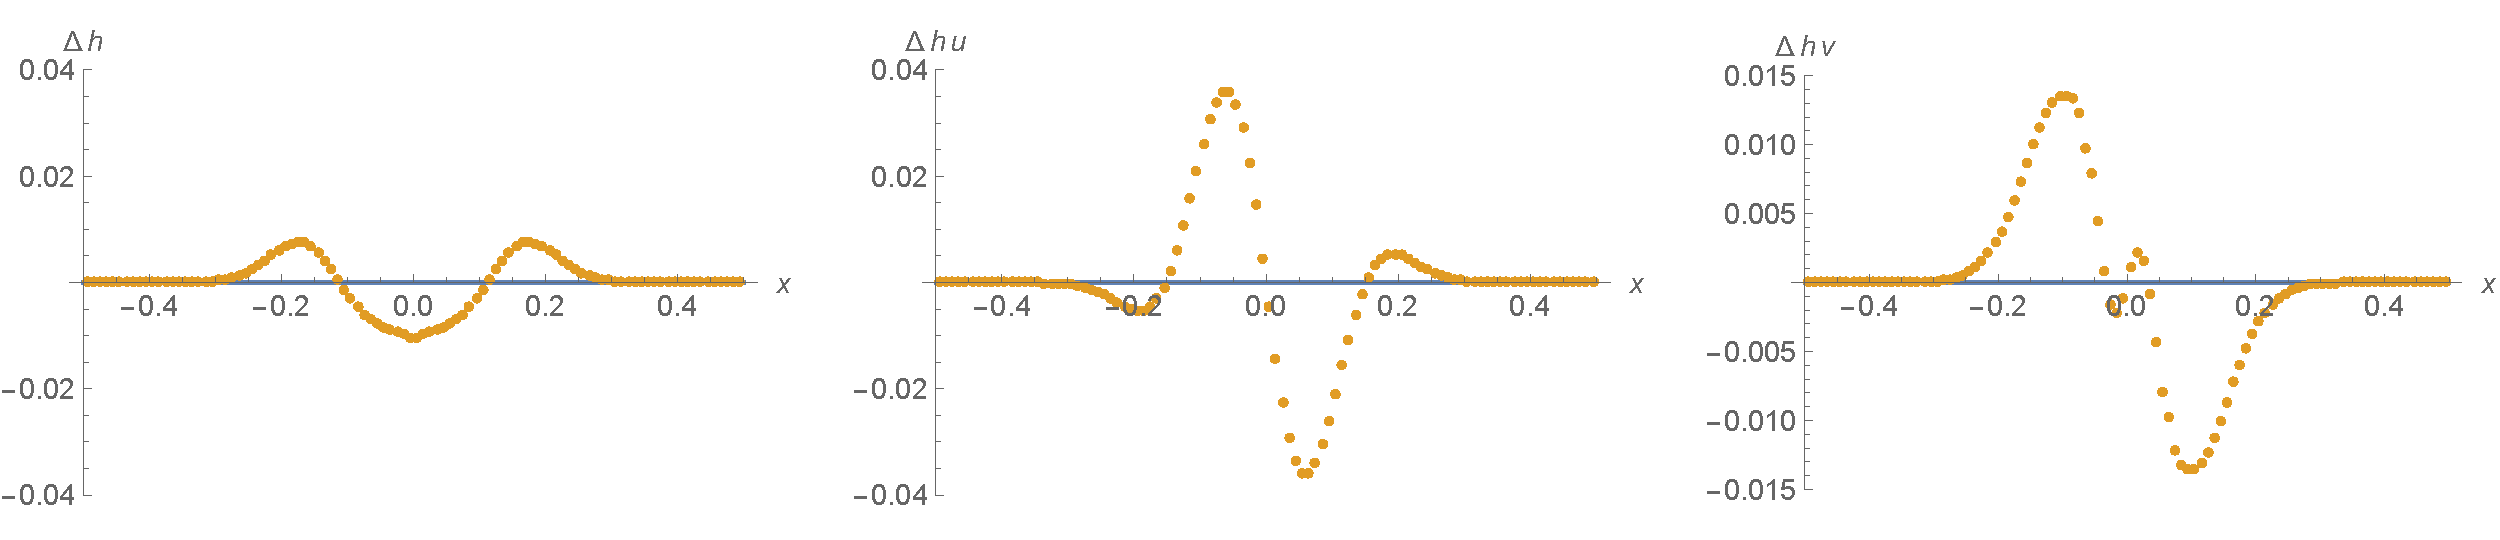
\includegraphics[width=\textwidth]{diagrams/results-geo-gauss-1}
    \caption{$t = 0.1$}
    \label{fig:results-geo-gauss-1}
  \end{subfigure} \\
  \begin{subfigure}{\textwidth}
    %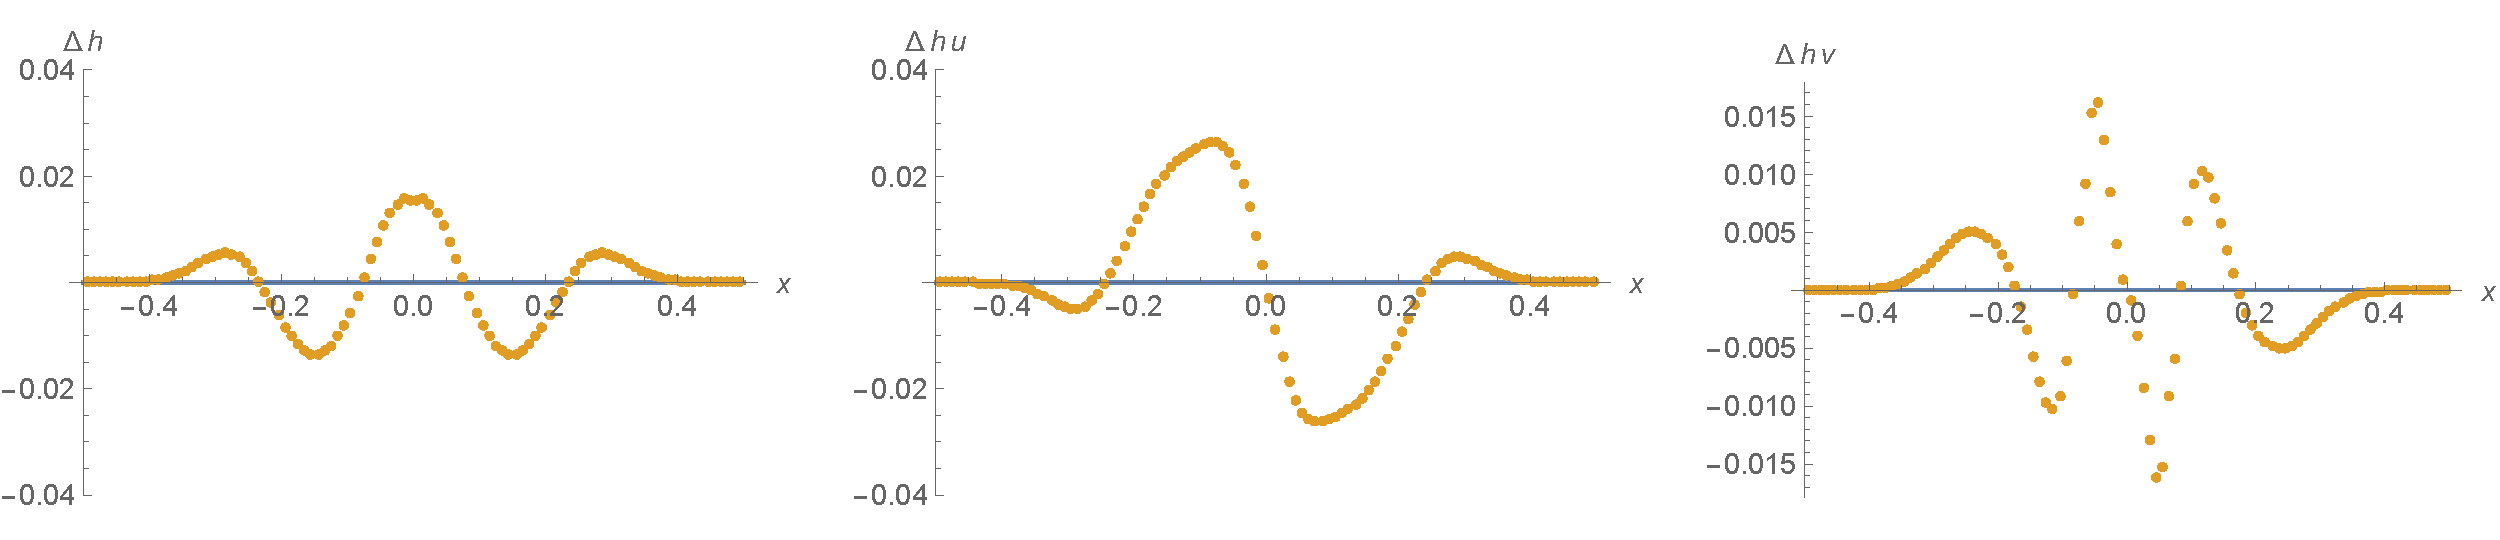
\includegraphics[width=\textwidth]{diagrams/results-geo-gauss-2}
    \caption{$t = 0.2$}
    \label{fig:results-geo-gauss-2}
  \end{subfigure} \\
  \begin{subfigure}{\textwidth}
    %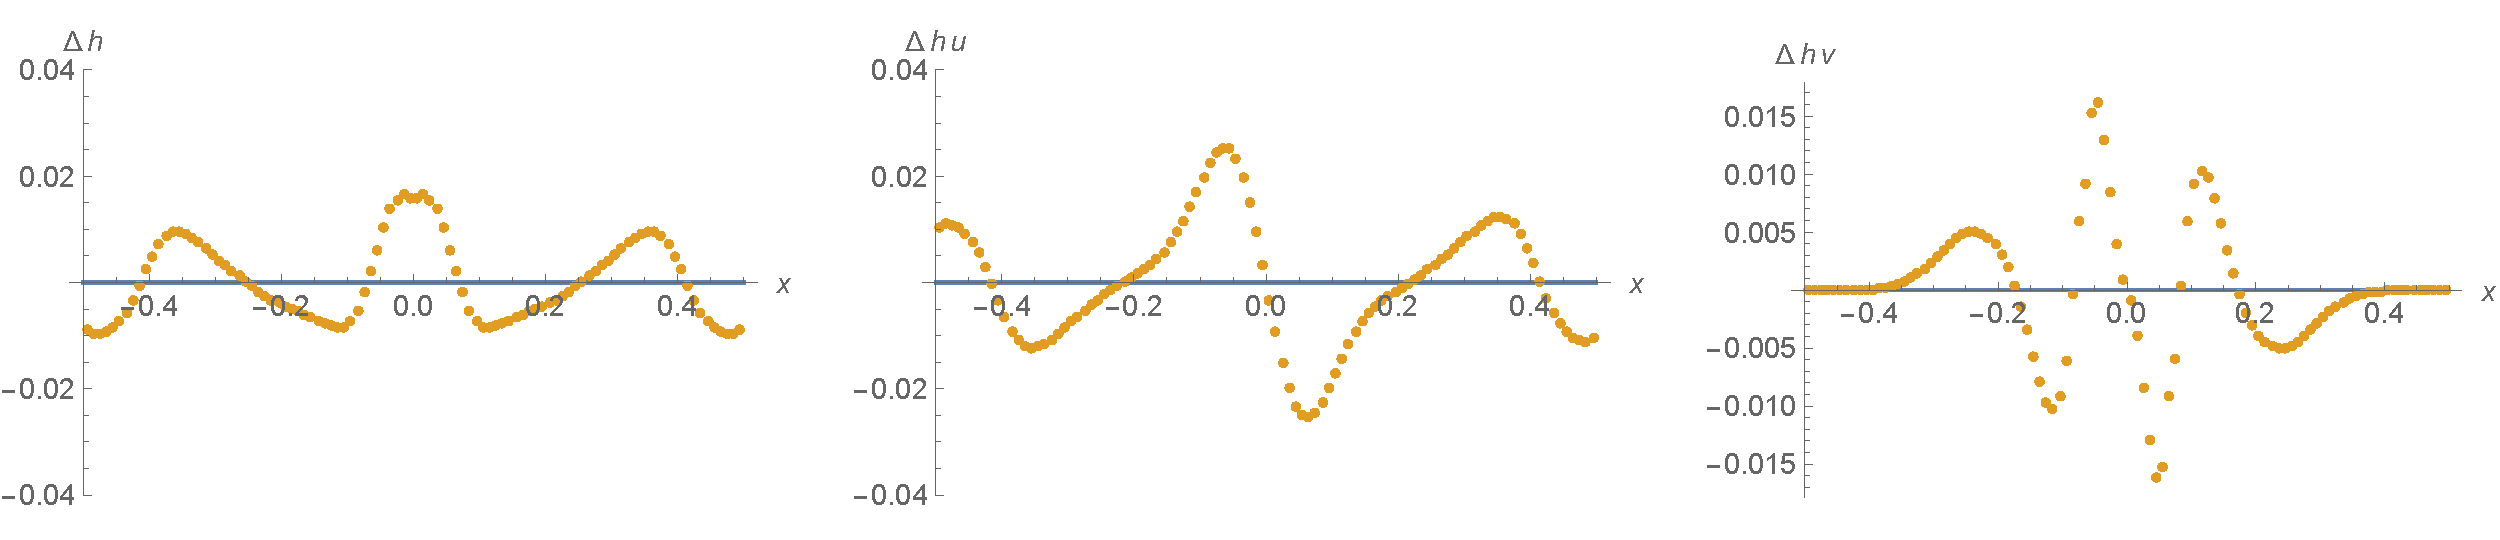
\includegraphics[width=\textwidth]{diagrams/results-geo-gauss-5}
    \caption{$t = 0.5$}
    \label{fig:results-geo-gauss-5}
  \end{subfigure} \\
  \begin{subfigure}{\textwidth}
    %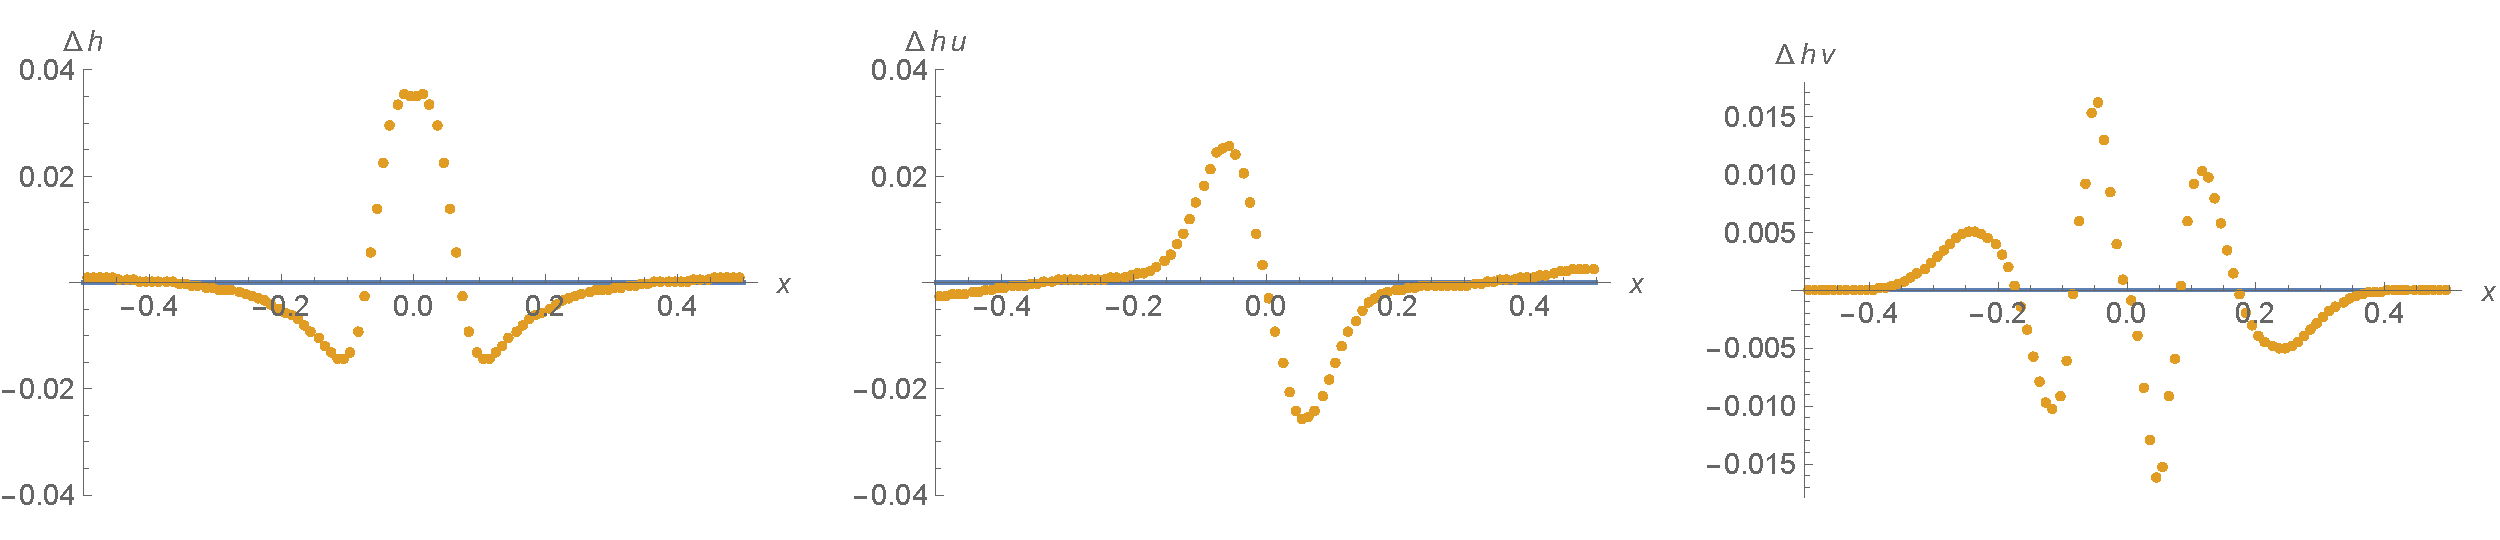
\includegraphics[width=\textwidth]{diagrams/results-geo-gauss-10}
    \caption{$t = 1.0$}
    \label{fig:results-geo-gauss-10}
  \end{subfigure}
  \caption{Results for geostrophic equilibrium over Gaussian bathymetry. The equilibrium state has been subtracted off the plots, such that the exact solution is $\Delta h = \Delta hu = \Delta hv = 0$. The data points correspond to the Rogers solver for still water systems over 100 grid cells. The columns correspond to the deviations of the conserved variables $h$, $hu$ and $hv$ and the rows to different time levels. $K = 10$.}
  \label{fig:results-geo-gauss}
\end{figure}

The results for geostrophic equilibrium (with Gaussian surface profile) over flat bathymetry is shown in Figs.~\ref{fig:results-geo}. As opposed to the previous two systems, these plots show only deviations from the equilibrium state, since errors would be barely visible otherwise.

The unbalanced solver and the Rogers solver for still water systems give identical results. This was to be expected, as the Coriolis term is unchanged for this solver. The magnitude of the generated waves is comparable to the still water case. This is also not surprising, as the gradients of $h$ are on the same order for both setups.

Both the LeVeque solver and the Rogers solver for geostrophic equilibria preserve the state exactly, as desired. Note that, as in the still water case, only for the Rogers solver are the deviations exactly zero. The LeVeque solver preserves the equilibrium to machine precision.

As mentioned in the previous chapter, one can also look at the balance between bathymetry and Coriolis terms by choosing the same (Gaussian) profile for bathymetry and water surface. In this case, the unbalanced, LeVeque and Rogers solver for geostrophic equilibria preserve the balance. In the case of the unbalanced solver this is due to both terms being computed in the same step and cancelling to machine precision. For the other two solvers it is simply a consequence of being able to maintain the balance of any geostrophic equilibrium. However, the Rogers solver for still water systems does not preserve this equilibrium as can be seen in Figs.~\ref{fig:results-geo-gauss}. Furthermore, it appears that the amplitude of $\Delta h$ grows without bounds albeit slowly. The author has not been able to determine whether this is due to an implementation detail (e.g. an inconsistent discretisation of bathymetry and initial conditions) or an inherent problem of the method.

\section{Wave through Geostrophic Equilibrium}

\begin{figure}
  \centering
  \begin{subfigure}{\textwidth}
    %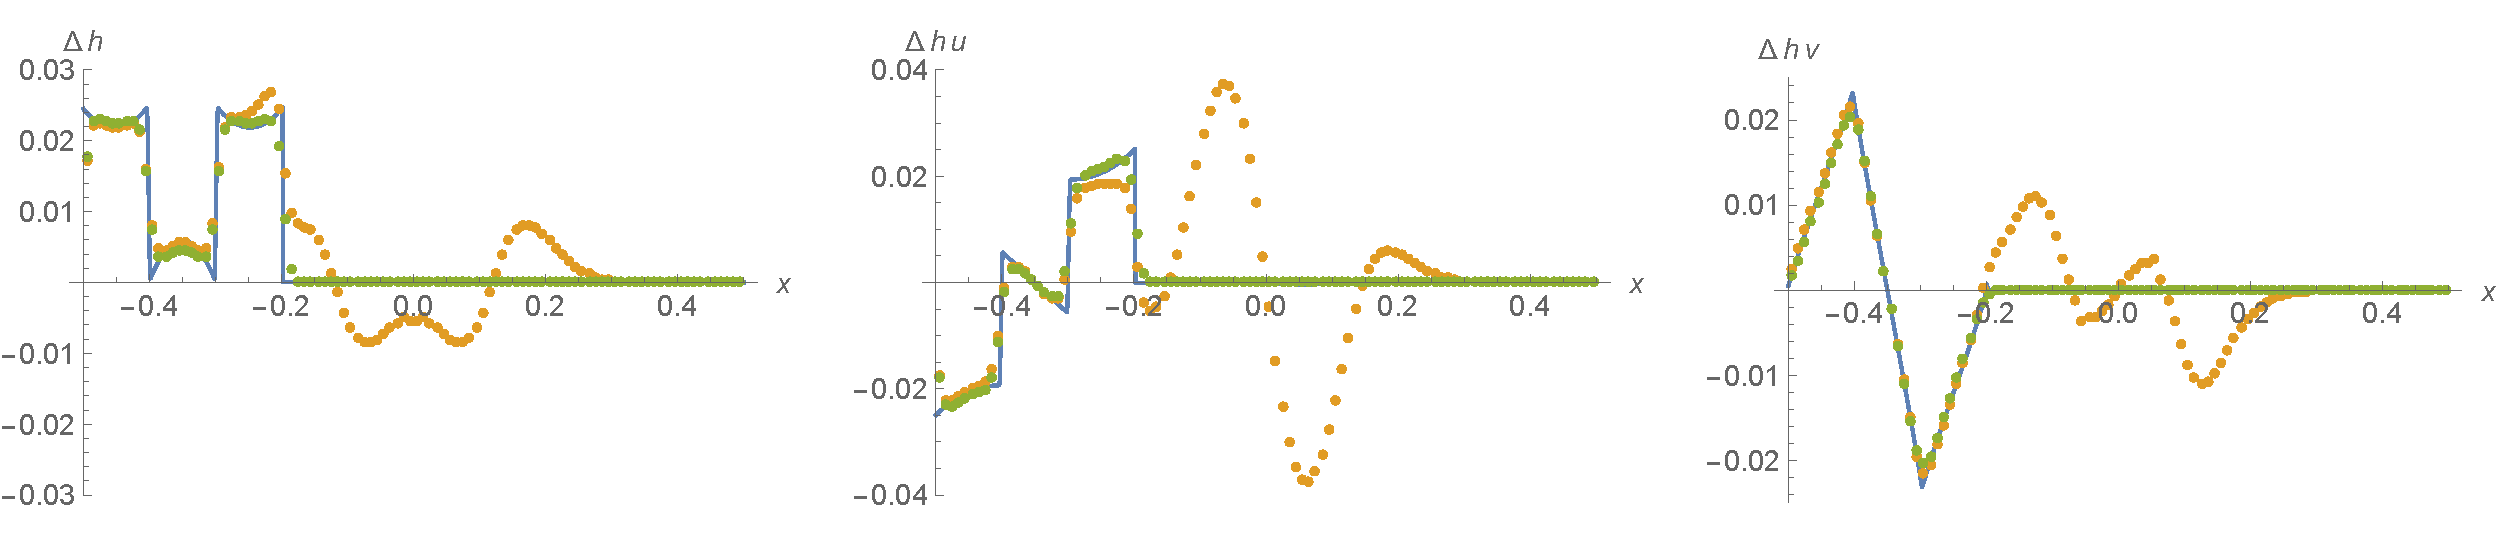
\includegraphics[width=\textwidth]{diagrams/results-geo-wave-1}
    \caption{$t = 0.1$}
    \label{fig:results-geo-wave-1}
  \end{subfigure} \\
  \begin{subfigure}{\textwidth}
    %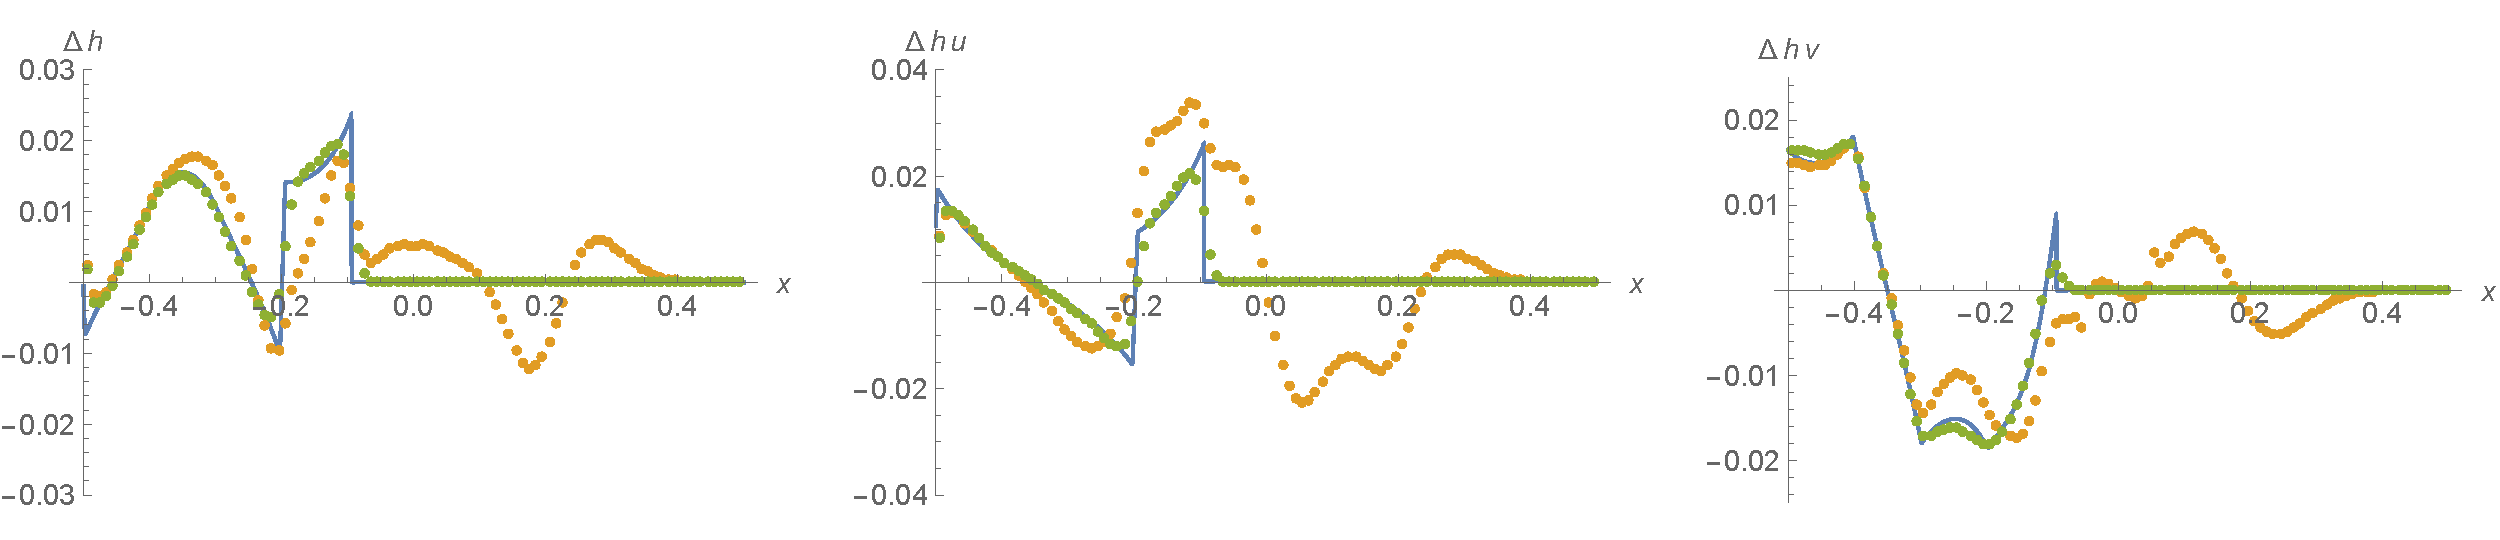
\includegraphics[width=\textwidth]{diagrams/results-geo-wave-2}
    \caption{$t = 0.2$}
    \label{fig:results-geo-wave-2}
  \end{subfigure} \\
  \begin{subfigure}{\textwidth}
    %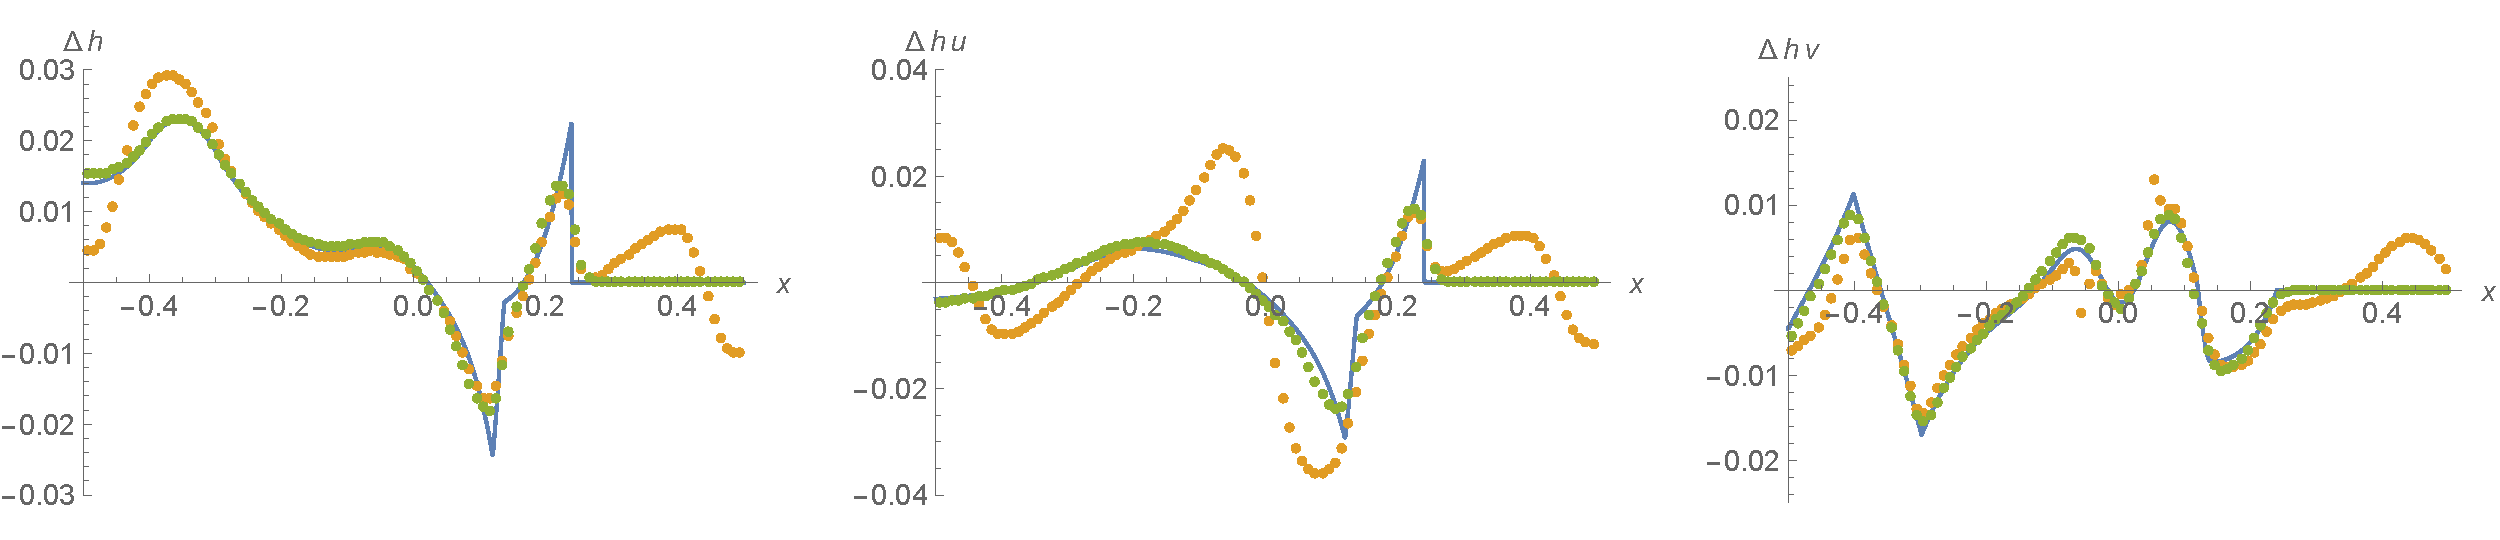
\includegraphics[width=\textwidth]{diagrams/results-geo-wave-5}
    \caption{$t = 0.5$}
    \label{fig:results-geo-wave-5}
  \end{subfigure} \\
  \begin{subfigure}{\textwidth}
    %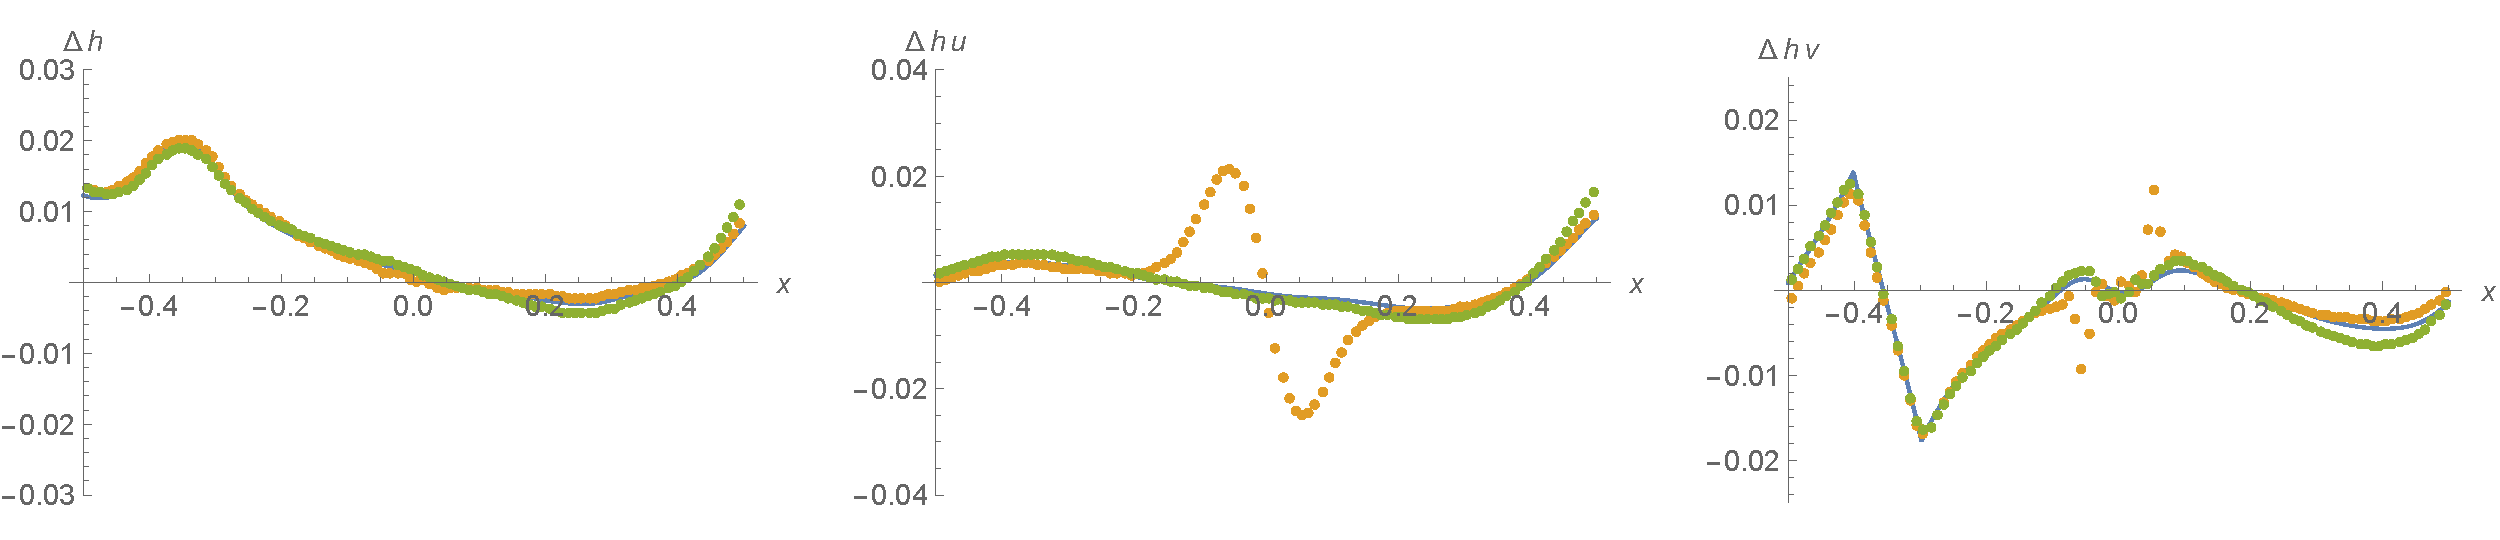
\includegraphics[width=\textwidth]{diagrams/results-geo-wave-10}
    \caption{$t = 1.0$}
    \label{fig:results-geo-wave-10}
  \end{subfigure}
  \caption{Results for wave through a geostrophic equilibrium. The equilibrium state has been subtracted off the plots. The reference solution has been computed with the unbalanced solver on 10000 grid cells and is shown as a solid blue line. The orange data was obtained with the unbalanced solver over 100 grid cells. The green data corresponds to the LeVeque solver. The columns correspond to the deviations of the conserved variables $h$, $hu$ and $hv$ and the rows to different time levels. $K = 10$.}
  \label{fig:results-geo-wave}
\end{figure}

\begin{figure}
  \centering
  \begin{subfigure}{\textwidth}
    %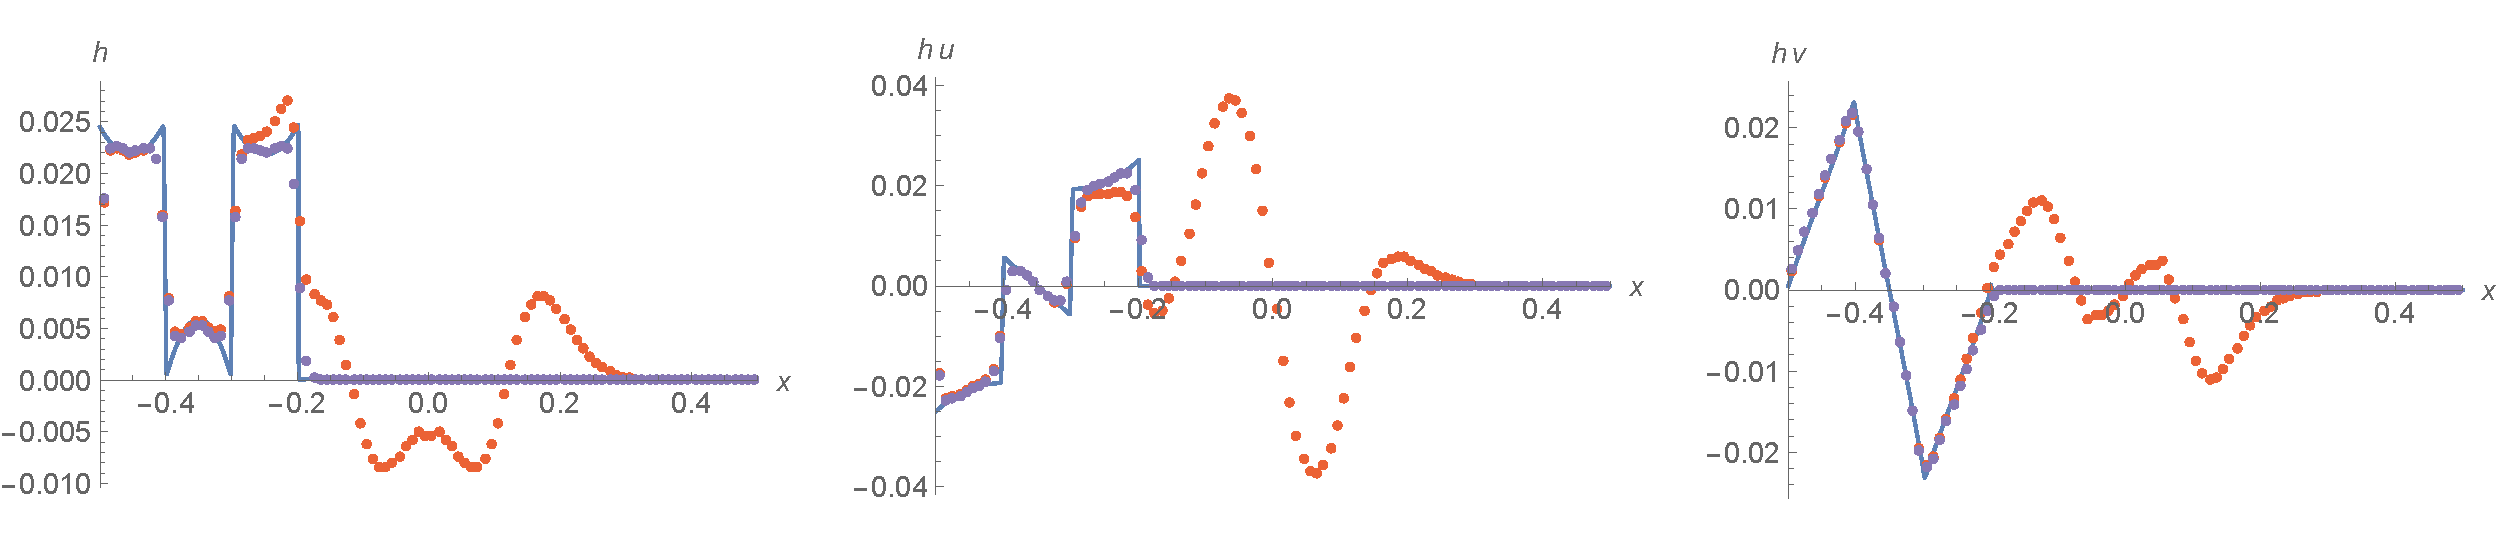
\includegraphics[width=\textwidth]{diagrams/results-geo-wave-rog-1}
    \caption{$t = 0.1$}
    \label{fig:results-geo-wave-rog-1}
  \end{subfigure} \\
  \begin{subfigure}{\textwidth}
    %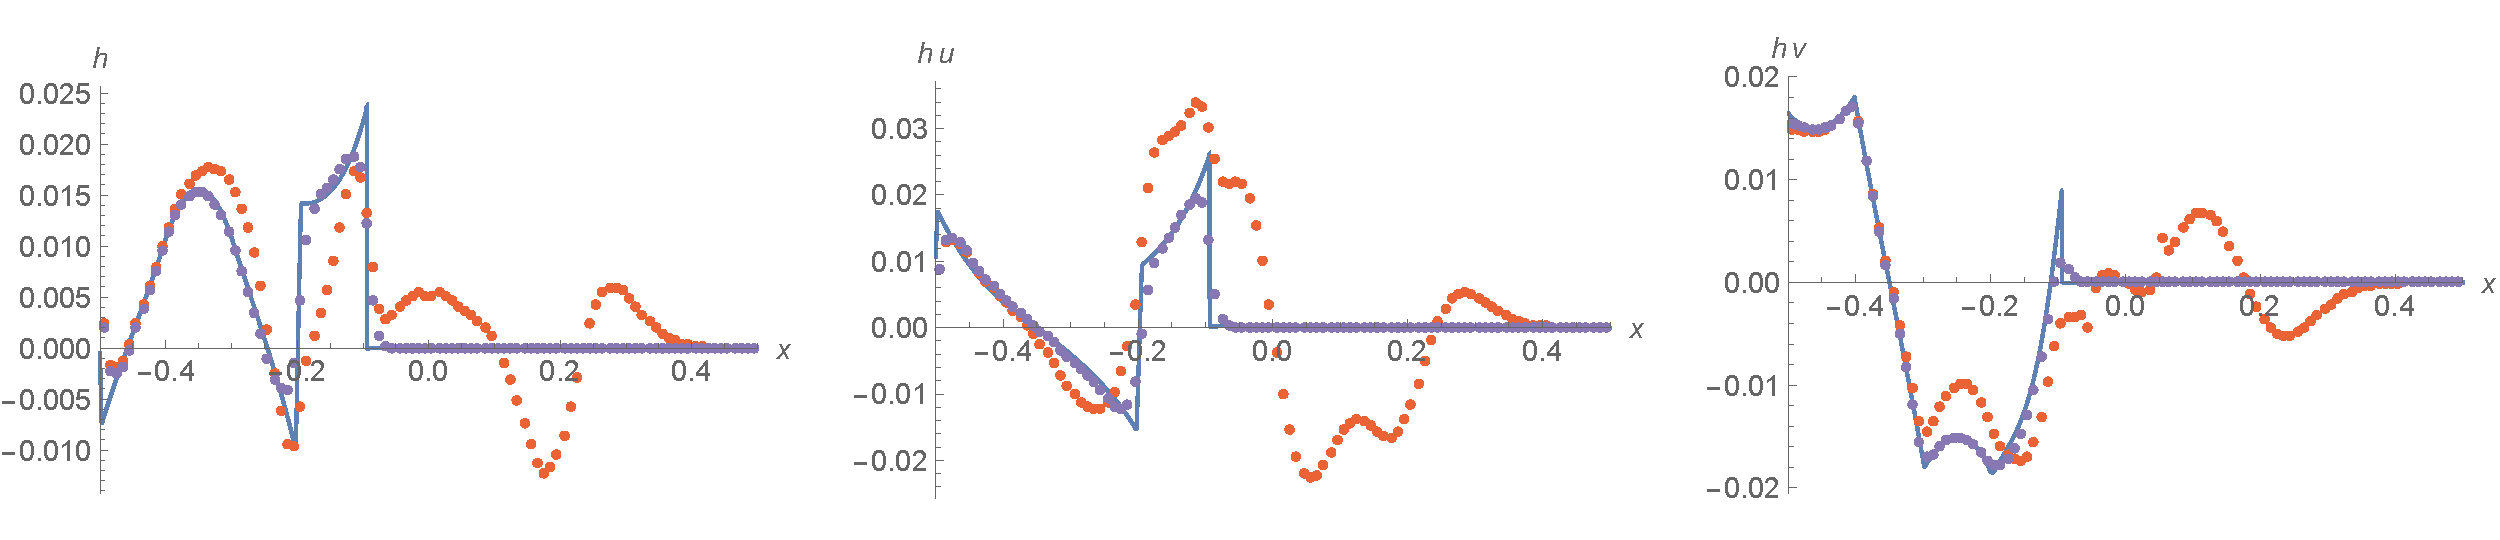
\includegraphics[width=\textwidth]{diagrams/results-geo-wave-rog-2}
    \caption{$t = 0.2$}
    \label{fig:results-geo-wave-rog-2}
  \end{subfigure} \\
  \begin{subfigure}{\textwidth}
    %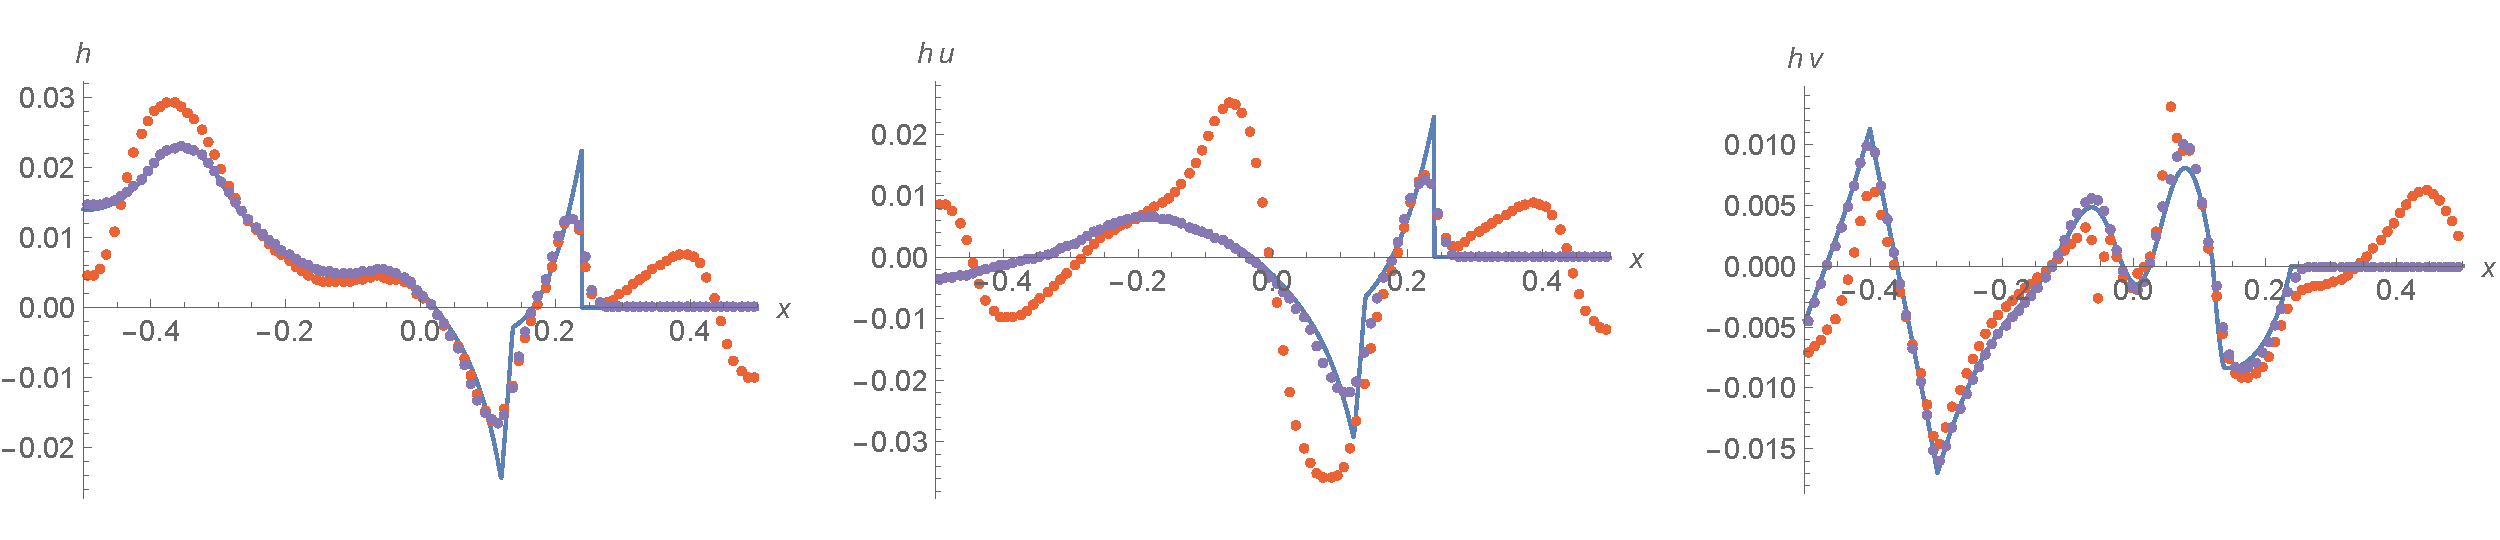
\includegraphics[width=\textwidth]{diagrams/results-geo-wave-rog-5}
    \caption{$t = 0.5$}
    \label{fig:results-geo-wave-rog-5}
  \end{subfigure} \\
  \begin{subfigure}{\textwidth}
    %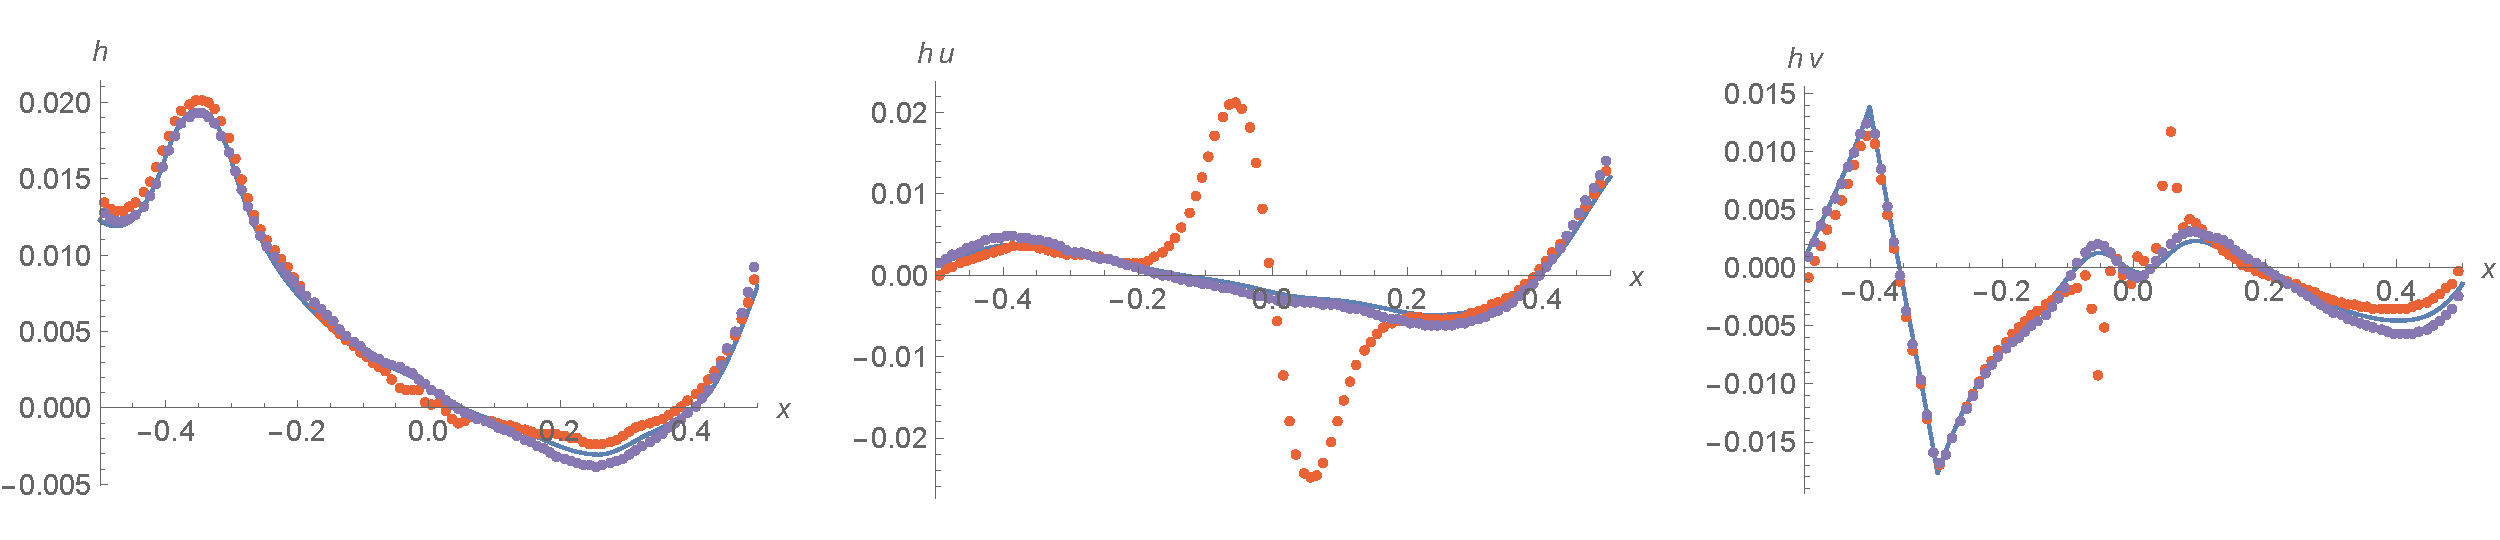
\includegraphics[width=\textwidth]{diagrams/results-geo-wave-rog-10}
    \caption{$t = 1.0$}
    \label{fig:results-geo-wave-rog-10}
  \end{subfigure}
  \caption{Results for wave through a geostrophic equilibrium. The equilibrium state has been subtracted off the plots. The reference solution has been computed with the unbalanced solver on 10000 grid cells and is shown as a solid blue line. The red data was obtained with the Rogers solver for still water systems over 100 grid cells. The blue data corresponds to the Rogers solver for geostrophic equilibria. The columns correspond to the deviations of the conserved variables $h$, $hu$ and $hv$ and the rows to different time levels. $K = 10$.}
  \label{fig:results-geo-wave-rog}
\end{figure}

This system is analogous to the wave through still water. It consists of a small perturbation added to the geostrophic equilibrium over flat bathymetry. The results for the unbalanced and LeVeque solver are shown in Figs.~\ref{fig:results-geo-wave}, those for the Rogers solvers in Figs.~\ref{fig:results-geo-wave-rog}. As before, the reference solution has been computed with the unbalanced solver on a fine grid with $N = 10000$.

It can be seen that the solvers which can preserve the geostrophic equilibrium itself (LeVeque and Rogers for geostrophic equilibria) also perform very well on this perturbed system, whereas the other unphysical waves generated by the other two solvers are comparable with the real waves again, which makes the results unreliable.

\section{Uniform Flow}

\begin{figure}
  \centering
  \begin{subfigure}{\textwidth}
    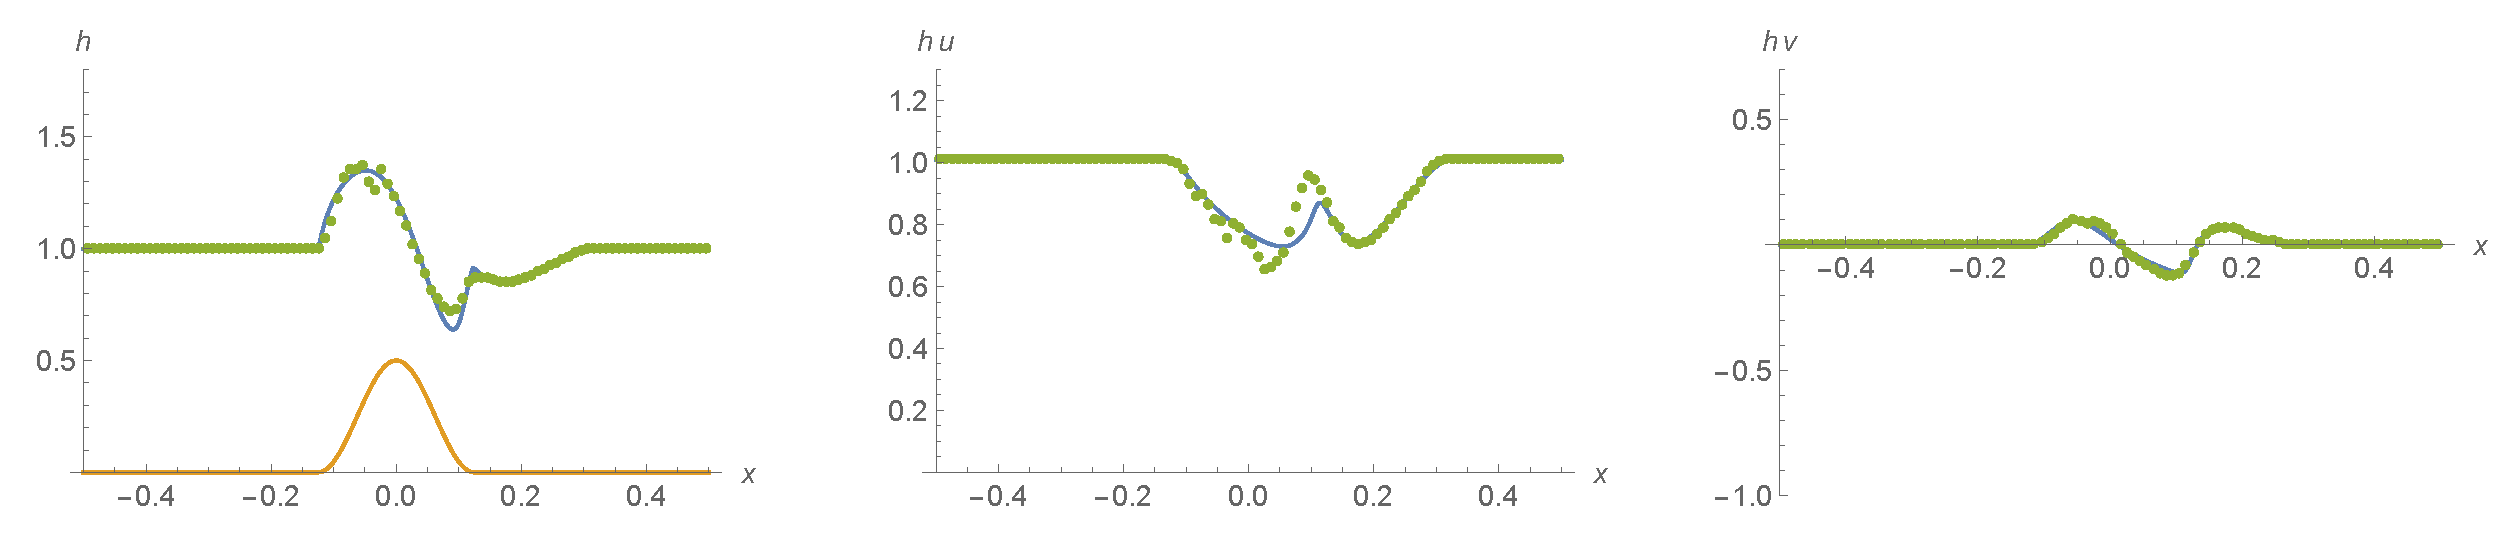
\includegraphics[width=\textwidth]{diagrams/results-flow-1}
    \caption{$t = 0.1$}
    \label{fig:results-flow-1}
  \end{subfigure} \\
  \begin{subfigure}{\textwidth}
    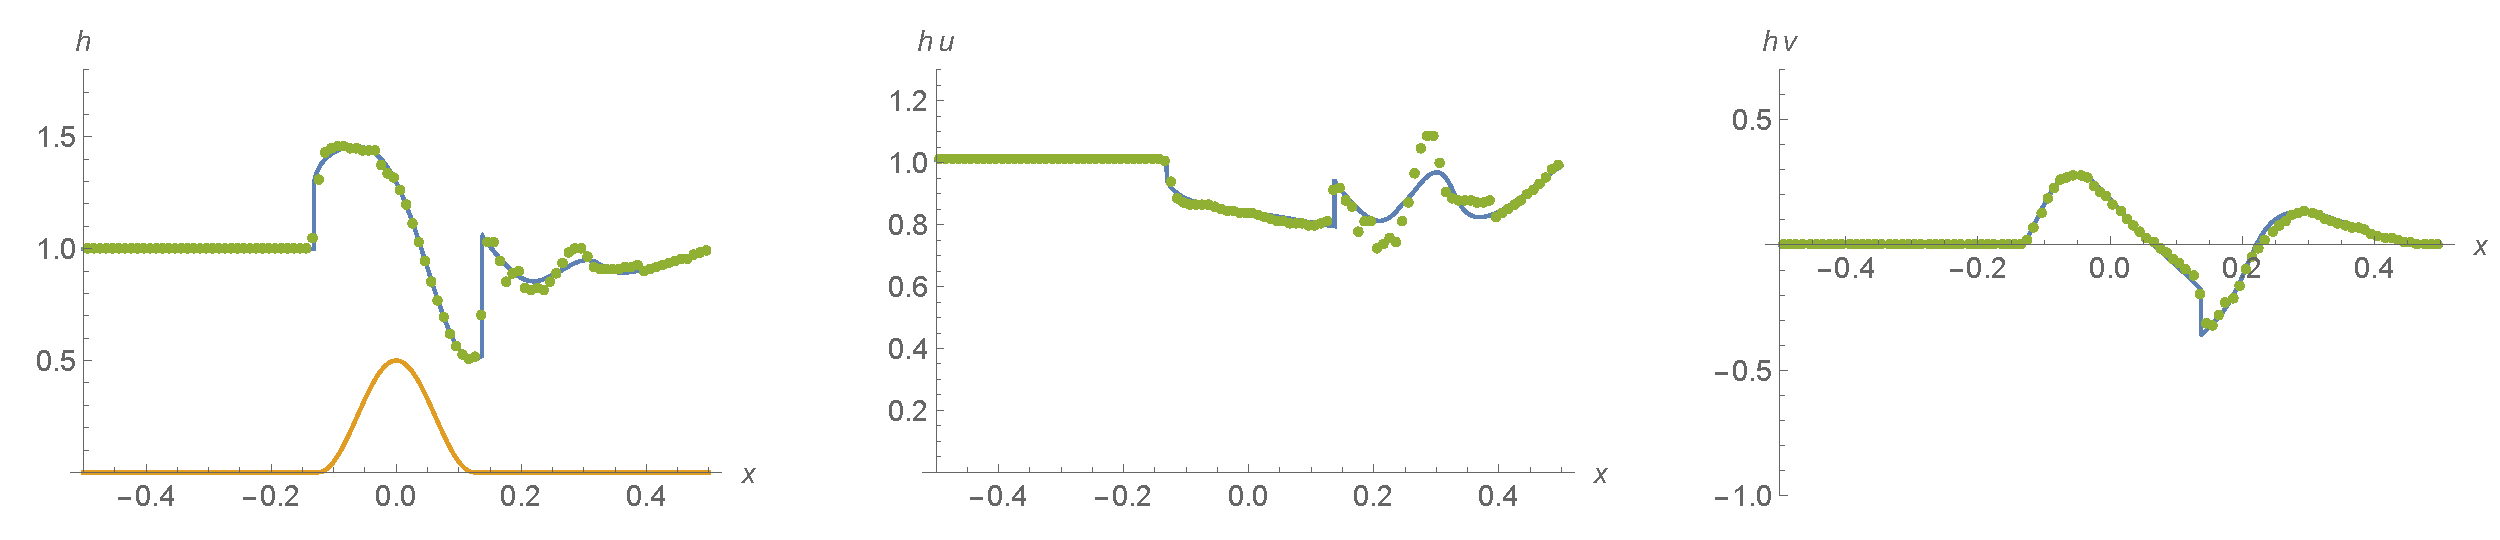
\includegraphics[width=\textwidth]{diagrams/results-flow-2}
    \caption{$t = 0.2$}
    \label{fig:results-flow-2}
  \end{subfigure} \\
  \begin{subfigure}{\textwidth}
    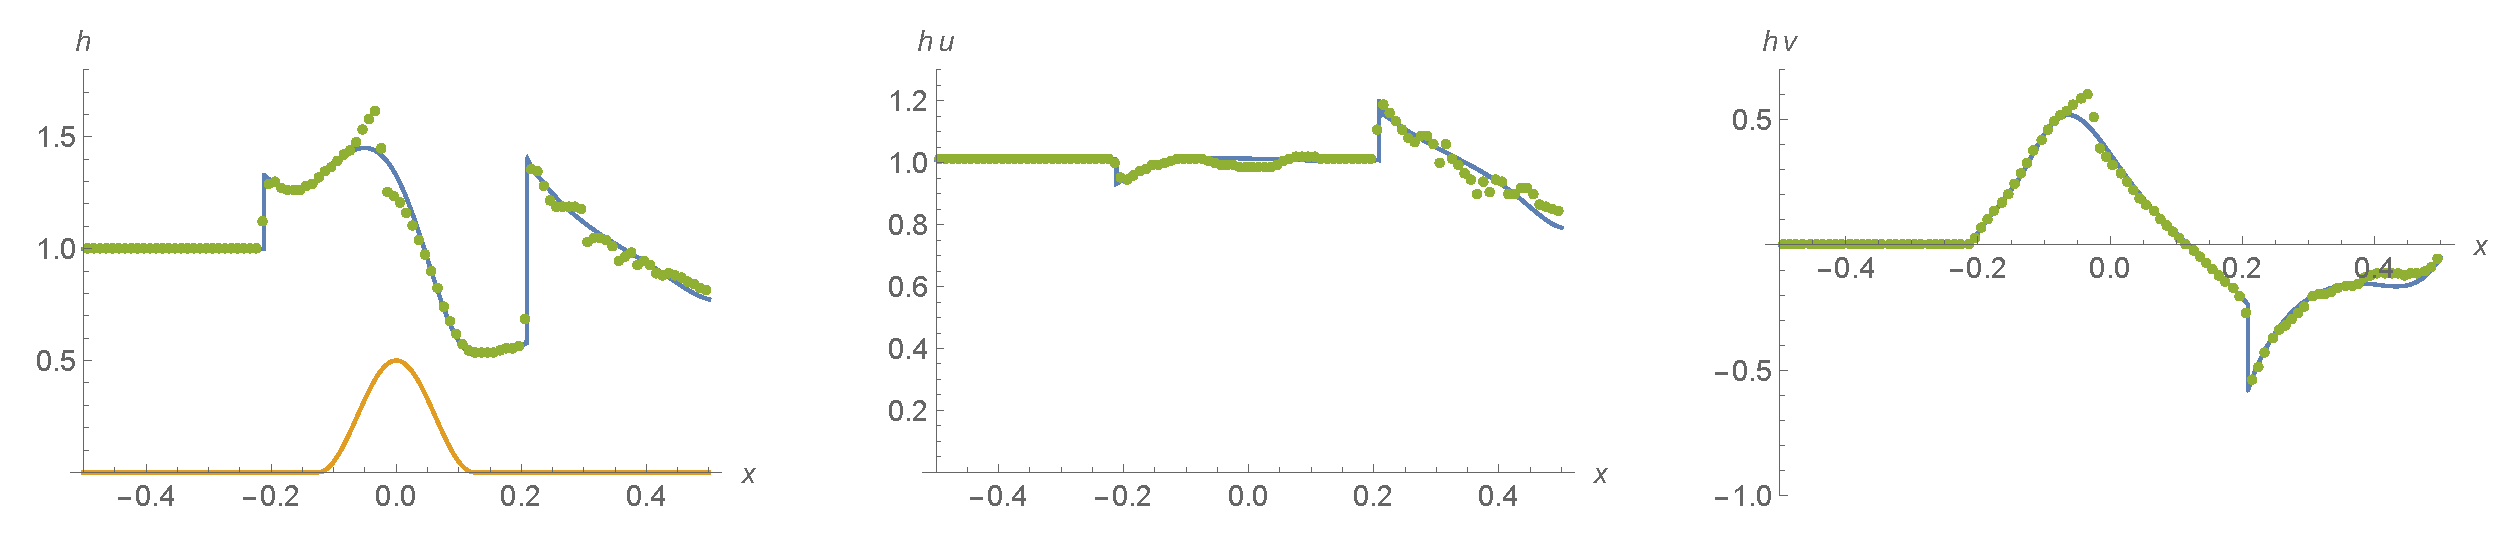
\includegraphics[width=\textwidth]{diagrams/results-flow-5}
    \caption{$t = 0.5$}
    \label{fig:results-flow-5}
  \end{subfigure} \\
  \begin{subfigure}{\textwidth}
    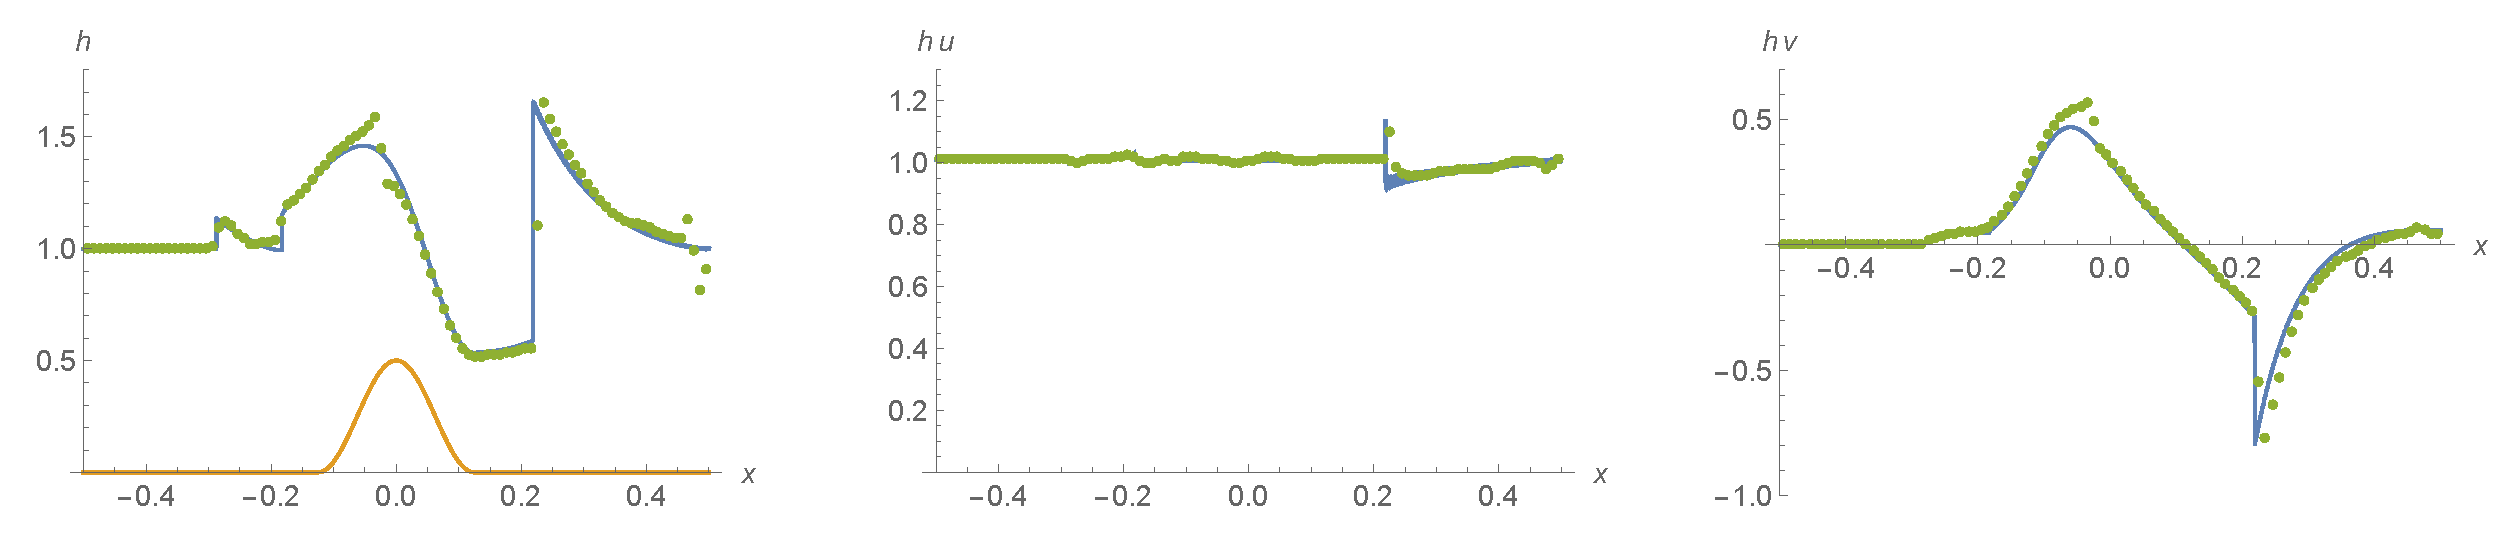
\includegraphics[width=\textwidth]{diagrams/results-flow-10}
    \caption{$t = 1.0$}
    \label{fig:results-flow-10}
  \end{subfigure}
  \caption{Results for transcritical flow over a cosine ridge. The reference solution has been computed with the unbalanced solver on 10000 grid cells and is shown as a solid blue line. The orange line represents the bathymetry. The green data was obtained with the LeVeque solver over 100 grid cells. The columns correspond to the deviations of the conserved variables $h$, $hu$ and $hv$ and the rows to different time levels. $K = 10$.}
  \label{fig:results-flow}
\end{figure}

When the system starts with uniform velocity in subcritical or supercritical flow, all methods were found to produce qualitatively correct (and converging) results, although the Rogers solvers seemed to be less accurate than the other two at low resolution.

However, the interesting case is transcritical flow. While the unbalanced and Rogers solvers can handle these cases as well as any uniform flow, the LeVeque solver fails to compute them correctly. This has already been observed in \citet{leveque1998balancing}. LeVeque found that the Newton method diverges when the shock forms over the bathymetry and suggested using an unbalanced method until an almost steady state is reached, and then switching to the balanced method.

The author has observed the same divergences but has not attempted switching methods. Instead, the Newton method was replaced by an explicit formula to solve the cubic equation (see \citet{press2007numerical}, pp. 178--179). While this stops the solution from breaking down, and the result roughly resembles the true solution, it contains too many shocks, as shown in Figs.~\ref{fig:results-flow}. Presumably, this is due to choosing the wrong root when all three roots are real. For some parameters and grid sizes these unphysical shocks can also grow large enough to violate the assumption that $h > 0$, in which case the solution also breaks down (as the solver has not been developed to support dry states).

\section{Execution Time}

\begin{itemize}
  \item show how unbalanced method fails
  \item go through different methods, showing where they work and where they fail
\end{itemize}